\chapter{Experimentos} % (fold)
\label{cha:experimentos}

Neste capítulo serão demonstrados os resultados obtidos com a utilização da metodologia apresentada.
Esta experimentação tem por objetivo expor a efetividade da técnica apresentada através de sua aplicação em diversos cenários.
Os experimentos realizados estão divididos em três categorias:
(i) um estudo quantitativo, que demonstra um conjunto de métricas e comparações entre casos distintos,
(ii) ambiente simulado no qual são utilizados agentes virtuais para realização do transporte, e
(iii) ambiente real, utilizando plataformas robóticas reais para transportar um objeto.

A metodologia apresentada foi totalmente implementada utilizando a linguagem de programação \emph{Python}\footnote{https://www.python.org/}, fazendo uso de algumas bibliotecas, tais como: \emph{networkx}, \emph{shapely}, \emph{descartes}, \emph{numpy}, \emph{sympy}, \emph{matplotlib}, dentre outras.
O computador utilizado durante os experimentos e simulações possui como configuração de \emph{hardware}: processador Intel Core i7-4500U CPU 1.80GHz*4, 8Gb de memória RAM, 128Gb SSD, Sistema Operacional Ubuntu 14.04, 64Bit.

\newpage

% subsection ambiente_de_programa_o (end)

% section arcabou_o_experimental (end)

\section{Estudo Quantitativo} % (fold)
\label{sec:estudo_quantitativo}

Nesta seção são discutidos os experimentos realizados com a utilização da técnica apresentada no Capítulo \ref{cha:metodologia}, com a finalidade de avaliar as características que influenciam a tarefa de transporte cooperativo, realizando diversas comparações sobre as possíveis configurações do sistema, como a complexidade do ambiente de trabalho, quantidade de objeto e robôs, e como estes dados refletem na mudança de comportamento do método.
Uma análise detalhada é apresentada em cada uma das próximas subseções, nas quais o elemento em estudo é sempre variável, enquanto demais características permanecem fixas, proporcionando um melhor entendimento de como uma certa propriedade influencia todo o sistema.

Inicialmente é apresentado um resultado para ilustração dos mapas e experimentos demonstrados a seguir.
Como mencionado anteriormente, o ambiente de trabalho do transporte é um espaço discretizado, formado por uma matriz de três dimensões, possuindo células de tamanho unitário.
Desta maneira, todos os experimentos que se referem ao deslocamento dentro do espaço, discutem a distância percorrida em unidades, ou seja, a quantidade de células a serem percorridas para realizar a movimentação de um ponto A para outro ponto B no mapa.
A Figura \ref{fig:result} demonstra um mapa de exemplo no qual um agente deve transportar um objeto. O trajeto vermelho é o plano criado para o objeto, partindo do ponto verde até a posição assinalada pelo ponto vermelho. O plano de movimentação do agente é demarcada por uma linha em azul, indicando todas as células percorridas pelo mesmo durante a execução da tarefa, que por exemplo, no primeiro plano de movimentação o agente percorreu um plano de tamanho 15.

\begin{figure}[htpb]
  \centering
  \setlength{\fboxsep}{0pt}
  \fbox{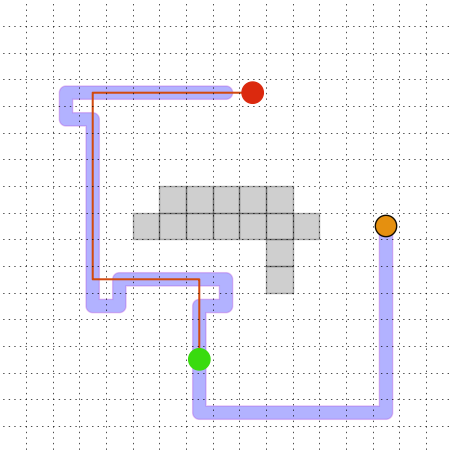
\includegraphics[width=0.42\textwidth]{img/experimentos/mapa_exemplo.png}}
  \caption[Mapa de exemplo do transporte de um objeto por um único agente]{Mapa de exemplo do transporte de um objeto por um único agente, destacando os trajetos realizados tanto pelo objeto quanto pelo agente.}
  \label{fig:result}
\end{figure}

\subsection{Complexidade do Ambiente} % (fold)
\label{sub:complexidade_do_ambiente}

Ao considerar que o transporte dos objetos sofre interferência direta do ambiente em que está sendo realizado, neste estudo, serão utilizados diferentes mapas, com variáveis níveis de complexidade e quantidade de obstáculos, apresentando como o sistema se comporta mediante estas diferentes circunstâncias.

A Figura \ref{fig:cenarios} apresenta exemplos de mapas utilizados nos experimentos desta seção.
Nestes cenários, a quantidade de objetos e robôs foi mantida fixa durante os experimentos (3 robôs e 3 objetos), havendo somente o incremento da complexidade do ambiente, possuindo mais obstáculos, com diferentes configurações.

A principal intenção deste experimento foi demonstrar que o sistema, além de ser capaz de tratar uma diversidade de mapas, não sofre uma grande influência da disposição dos obstáculos no ambiente, apesar de, inevitavelmente, um ambiente com grande restrição de movimentação contribuir em um aumento na distância percorrida pelos agentes.

\begin{figure}[h]
  \centering
  \setlength{\fboxsep}{0pt}
  \begin{subfigure}[t]{0.45\textwidth}
    \centering
    \fbox{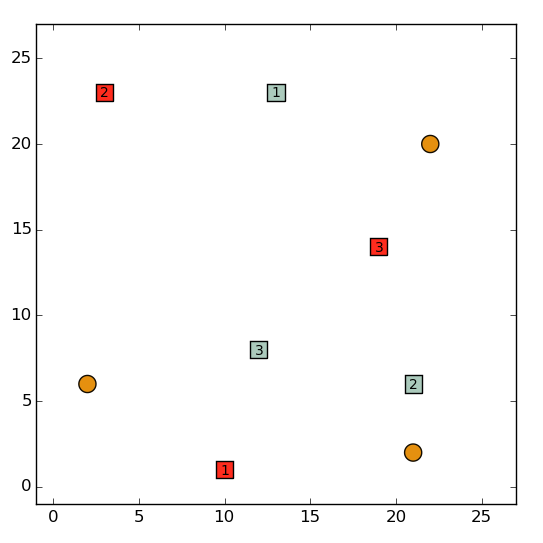
\includegraphics[width=\textwidth]{img/experimentos/ambient_1.png}}
    \caption{Ambiente sem obstáculos}
  \end{subfigure}
  \hspace{0.2cm}
  \begin{subfigure}[t]{0.45\textwidth}
    \centering
    \fbox{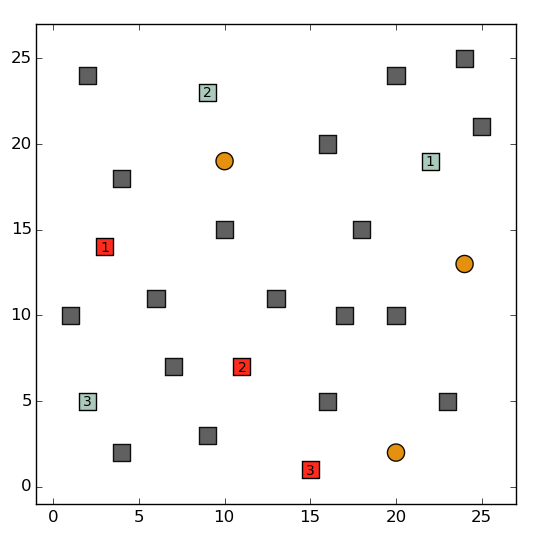
\includegraphics[width=\textwidth]{img/experimentos/ambient_2.png}}
    \caption{Ambiente com obstáculos dispersos.}
  \end{subfigure}

  \vspace{0.3cm}
  \begin{subfigure}[t]{0.45\textwidth}
    \centering
    \fbox{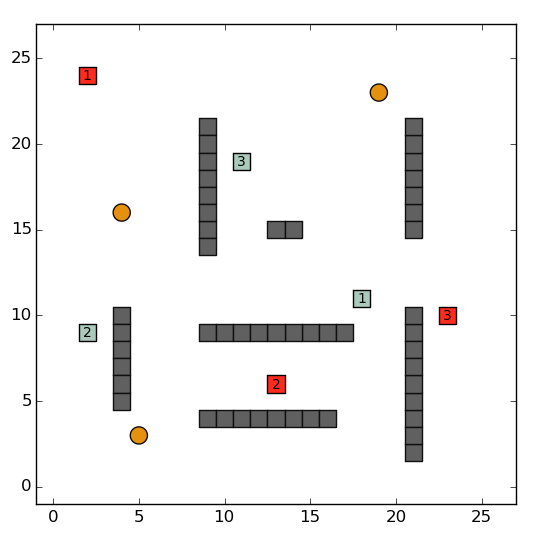
\includegraphics[width=\textwidth]{img/experimentos/ambient_3.png}}
    \caption{Ambiente com pouca restrição.}
  \end{subfigure}
  \hspace{0.2cm}
  \begin{subfigure}[t]{0.45\textwidth}
    \centering
    \fbox{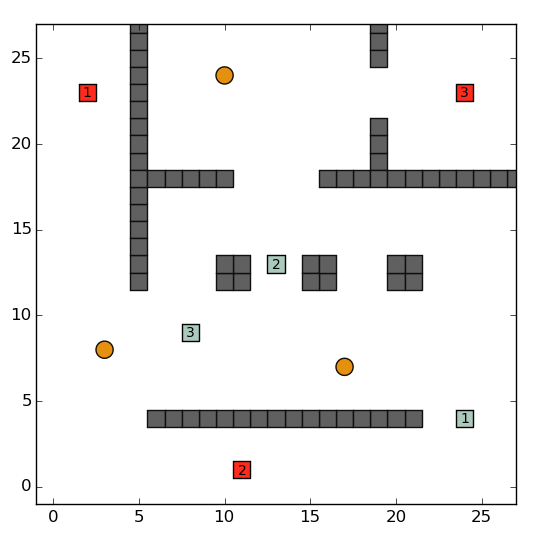
\includegraphics[width=\textwidth]{img/experimentos/ambient_4.png}}
    \caption{Ambiente com grande restrição.}
  \end{subfigure}

  \caption[Cenários utilizados nos experimentos relacionados à complexidade do ambiente]{Cenários utilizados nos experimentos relacionados à complexidade do ambiente. Os mapas foram criados buscando descrever cenários que possuam diferentes classes de mobilidade, partindo desde o exemplo onde não existem obstáculos, até outros que restringem drasticamente a movimentação tanto de objetos quanto agentes. Cada objeto é demarcado por um identificador numerado, descrevendo o ponto inicial (caixa azul) até seu respectivo destino (caixa vermelha). Os agentes são representados por círculos laranjas.}
  \label{fig:cenarios}
\end{figure}

Os experimentos realizados seguiram as seguintes regras: (i) cada cenário específico foi executado 10 vezes para obtenção dos dados relativos ao tempo médio de planejamento, e (ii) foram realizadas 3 variações aleatórias do posicionamento dos objetos e agentes dentro do ambiente para fins demonstrativos.

Os resultados dos experimentos realizados nestes ambientes podem ser vistos nos gráficos das figuras \ref{fig:cenarios_objeto}, \ref{fig:cenarios_robo}, que demonstram o deslocamento total dos objetos e agentes, respectivamente.
Como pode ser observado, o tamanho do plano de deslocamento dos objetos não segue diretamente um padrão relacionado a complexidade do ambiente, e principalmente à disposição dos mesmos, podendo haver um acréscimo ou descrésimo mediante a relação entre o ponto inicial e final.
O mesmo ocorre com o deslocamento dos robôs, que seguem um modelo similar ao plano dos objetos, quando os planos de transporte são reduzidos, a movimentação dos agentes também é reduzida.

Em contra-partida, o gráfico de tempo de planejamento, demonstrado na Figura \ref{fig:cenarios_tempo}, aponta para o aumento na demanda de tempo necessário durante o planejamento dos planos. Isso era esperado, porque em um ambiente mais restrito, o objeto geralmente deve realizar uma quantidade maior de mudanças de direção durante o transporte, influenciando a etapa de planejamento dos agentes, que devem criar mais planos para cada segmento.
Desta maneira, pode-se concluir que o ambiente certamente gera grande influência sobre o comportamento geral do sistema.

\begin{figure}[h]
  \centering
  \setlength{\fboxsep}{0pt}
  \fbox{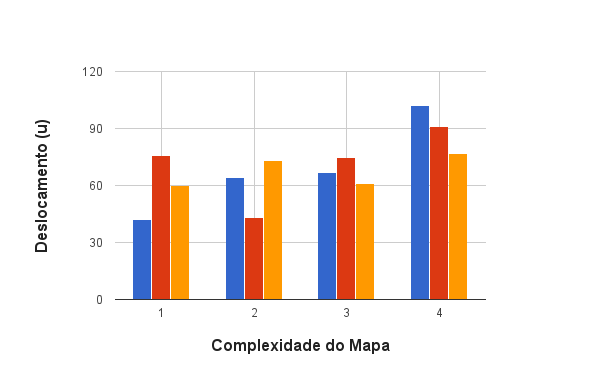
\includegraphics[width=0.55\textwidth]{img/experimentos/ambient_objeto.png}}
  \caption{Gráfico do deslocamento do objeto em ambiente com diferentes complexidades. São exemplificados três amostras onde os agentes são dispostos em posições diferentes.}
  \label{fig:cenarios_objeto}
\end{figure}

\begin{figure}[h]
  \centering
  \setlength{\fboxsep}{0pt}
  \fbox{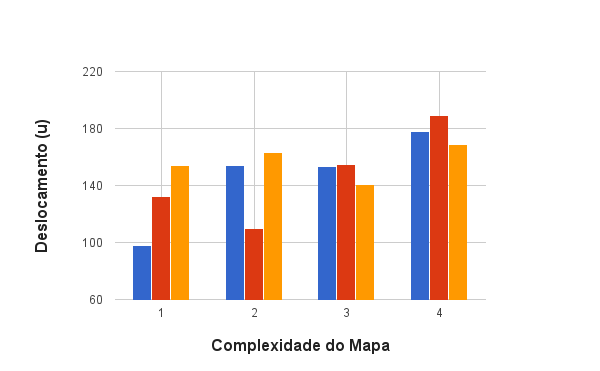
\includegraphics[width=0.55\textwidth]{img/experimentos/ambient_robo.png}}
  \caption{Gráfico de deslocamento dos agentes em cenários com variados graus de restrição de movimentos. Cada amostra demonstrada, representa cenários com agentes em posições distintas.}
  \label{fig:cenarios_robo}
\end{figure}

\begin{figure}[h]
  \centering
  \setlength{\fboxsep}{0pt}
  \fbox{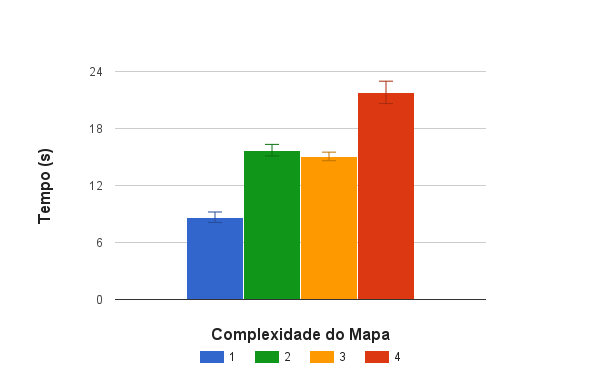
\includegraphics[width=0.55\textwidth]{img/experimentos/ambient_tempo.png}}
  \caption[Gráfico do tempo médio necessário para o planejamento total do sistema]{Gráfico do tempo médio necessário para o planejamento de todos os passos a serem executados durante o transporte em cenários com distintos níveis de complexidade.}
  \label{fig:cenarios_tempo}
\end{figure}

% subsection complexidade_do_ambiente (end)

\clearpage

\subsection{Deslocamento e Tempo de Planejamento dos Agentes} % (fold)
\label{sub:deslocamento_e_templo_de_planejamento_dos_agentes}

Para realizar um estudo específico do planejamento dos agentes, é utilizado um ambiente fixo de complexidade média, como o demonstrado na Figura \ref{fig:ambiente_penalizacao}. Será apresentado um conjunto de experimentos expondo a relação entre a quantidade de robôs e a quantidade de objetos a serem transportados.
Quanto maior a equipe, existe uma maior possibilidade de haver agentes mais aptos para o transporte, porém, como será demonstrado a seguir, em alguns casos, uma equipe maior prejudica a execução total.

% Tal relação se concentra na quantidade de opções (agentes) para transportar um determinado objeto.

\begin{figure}[htpb]
  \centering
  \setlength{\fboxsep}{0pt}
  \fbox{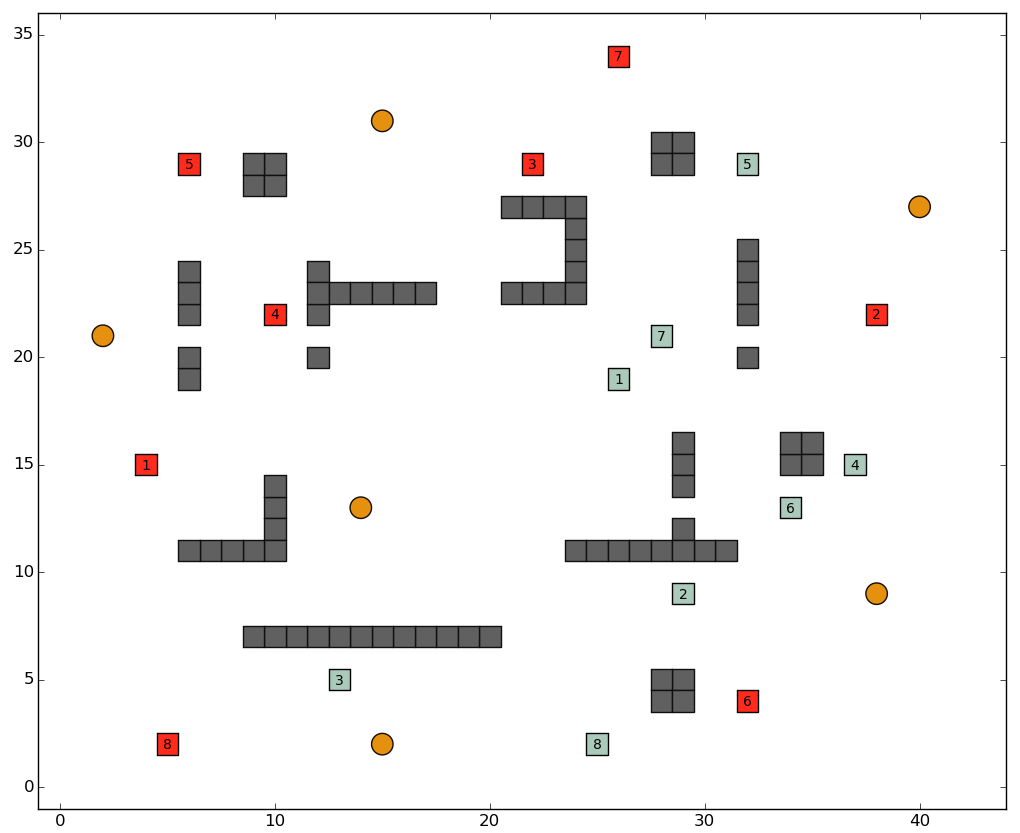
\includegraphics[width=0.5\textwidth]{img/experimentos/ambiente_penalizado.png}}
  \caption[Mapa utilizado nos testes de deslocamento e tempo de planejamento dos agentes]{Mapa utilizado nos testes de deslocamento e tempo de planejamento dos agentes. Neste caso específico, é exibida uma equipe com 6 agentes tendo de transportar 8 objetos dispersos no ambiente.}
  \label{fig:ambiente_penalizacao}
\end{figure}

Esta análise visa demonstrar como o sistema se beneficia do tamanho da equipe além de ilustrar o seu comportamento quando há um certo volume de objetos.
Os experimentos realizados contemplam equipes de 1 até 6 agentes, e o conjunto de objetos variando desde 1 até 8 itens.

Como discutido no Capítulo \ref{cha:metodologia}, o método aqui proposto aplica uma penalização nos planos criados para os objetos e agentes, sempre que existe uma mudança de direção, criando planos mais retilíneos, ou seja, planos que não alternam excessivamente a direção durante o transporte.
Esta penalização se mostrou importante no decorrer da manipulação, pois diminui a distância percorrida pelos agentes, além de minimizar o custo em tempo necessário para o planejamento.

% Exemplo

Para exemplificar visualmente esta diferença, que será discutida a seguir, são apresentados dois gráficos na Figura \ref{fig:ambiente_penalizacao_testes}, que ilustram somente o deslocamento de um agente para transportar 3 objetos, nos casos sem e com a penalização da mudança de direção.
Nos mapas existem 3 áreas destacadas, onde é possível perceber que no exemplo sem a penalidade (Figura \ref{fig:ambiente_penalizacao_sem}), o agente realiza uma série de mudanças de direção que não são realizadas no caso em que há a penalidade (Figura \ref{fig:ambiente_penalizacao_com}).
Desta maneira, o agente tende se deslocar menos durante todo a tarefa de transporte, além de conseguir completar a mesma tarefa em um menor tempo.

\begin{figure}[htpb]
  \centering
  \setlength{\fboxsep}{0pt}

  \begin{subfigure}[t]{0.45\textwidth}
    \centering
    \fbox{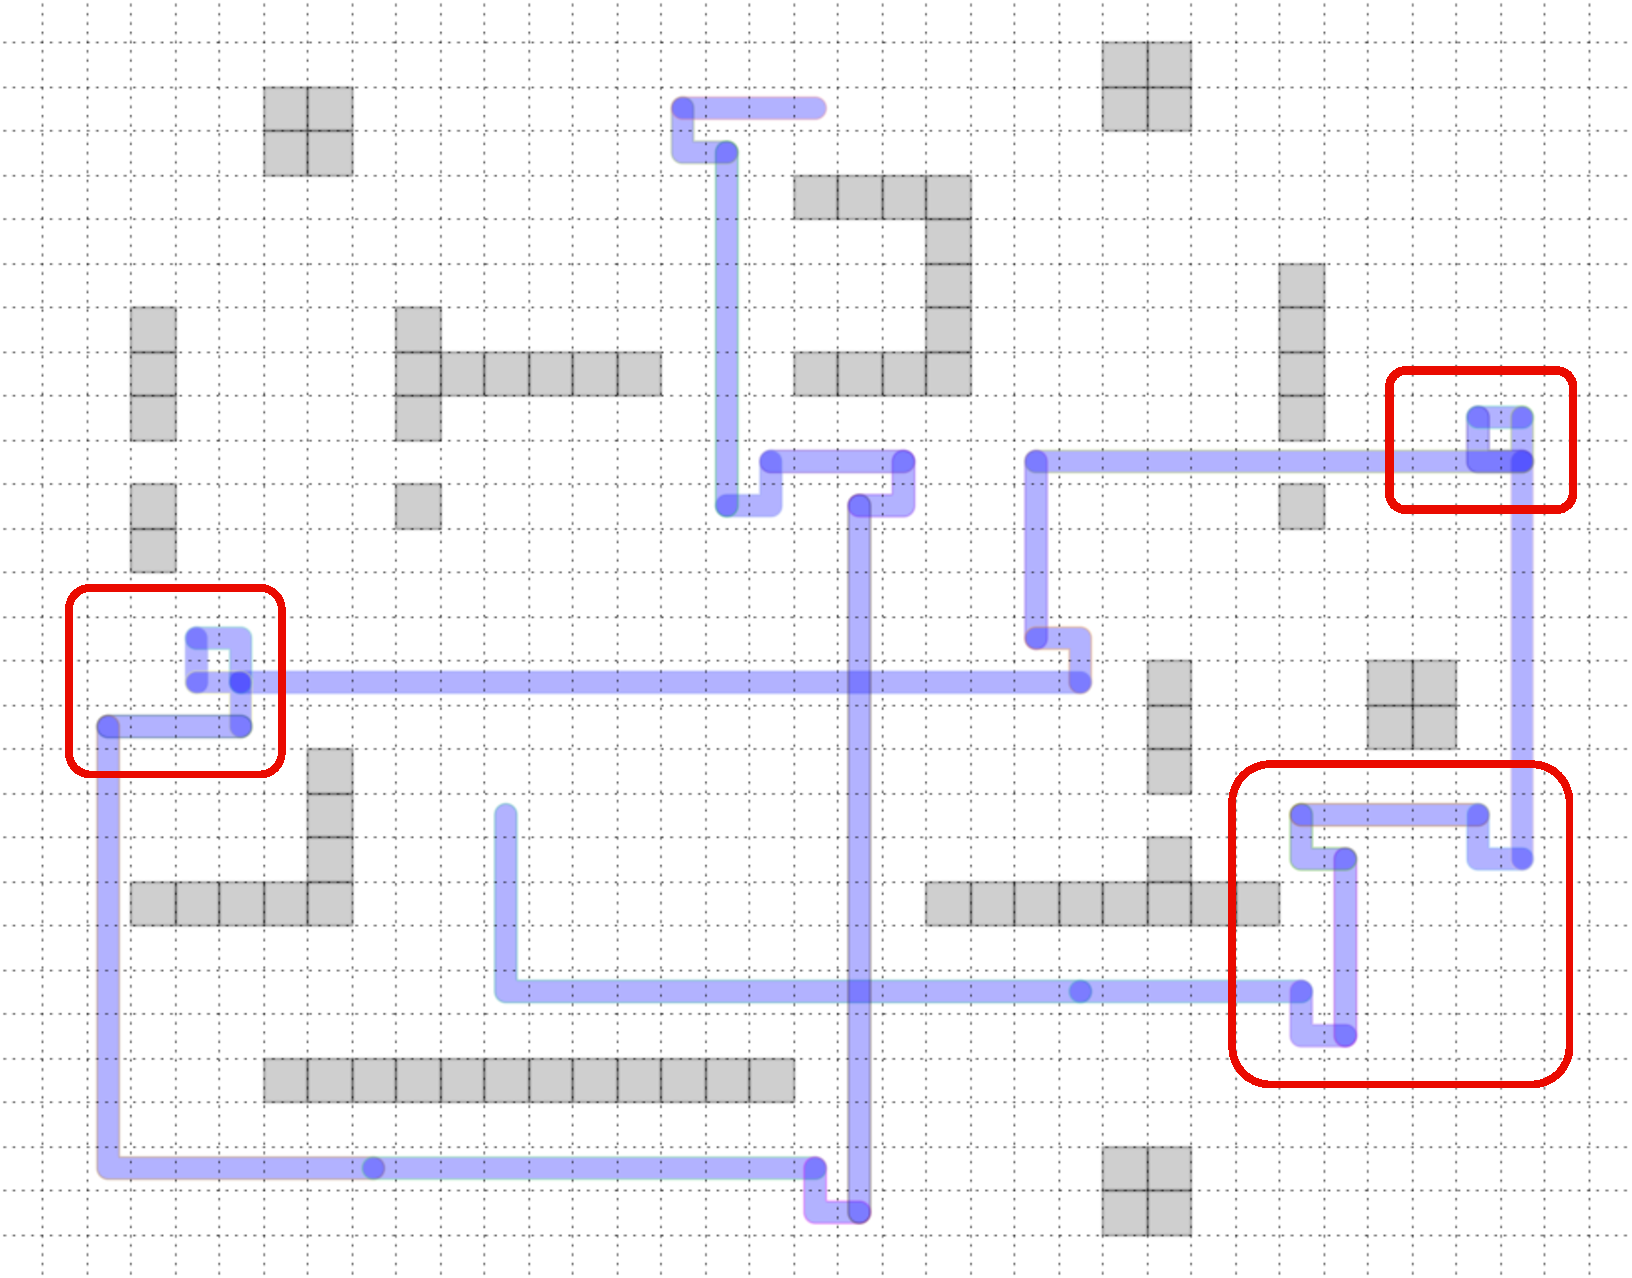
\includegraphics[width=\textwidth]{img/experimentos/ambiente_penalizacao_sem.pdf}}
    \caption{Exemplo sem a penalização.}
    \label{fig:ambiente_penalizacao_sem}
  \end{subfigure}
  \hspace{0.2cm}
  \begin{subfigure}[t]{0.45\textwidth}
    \centering
    \fbox{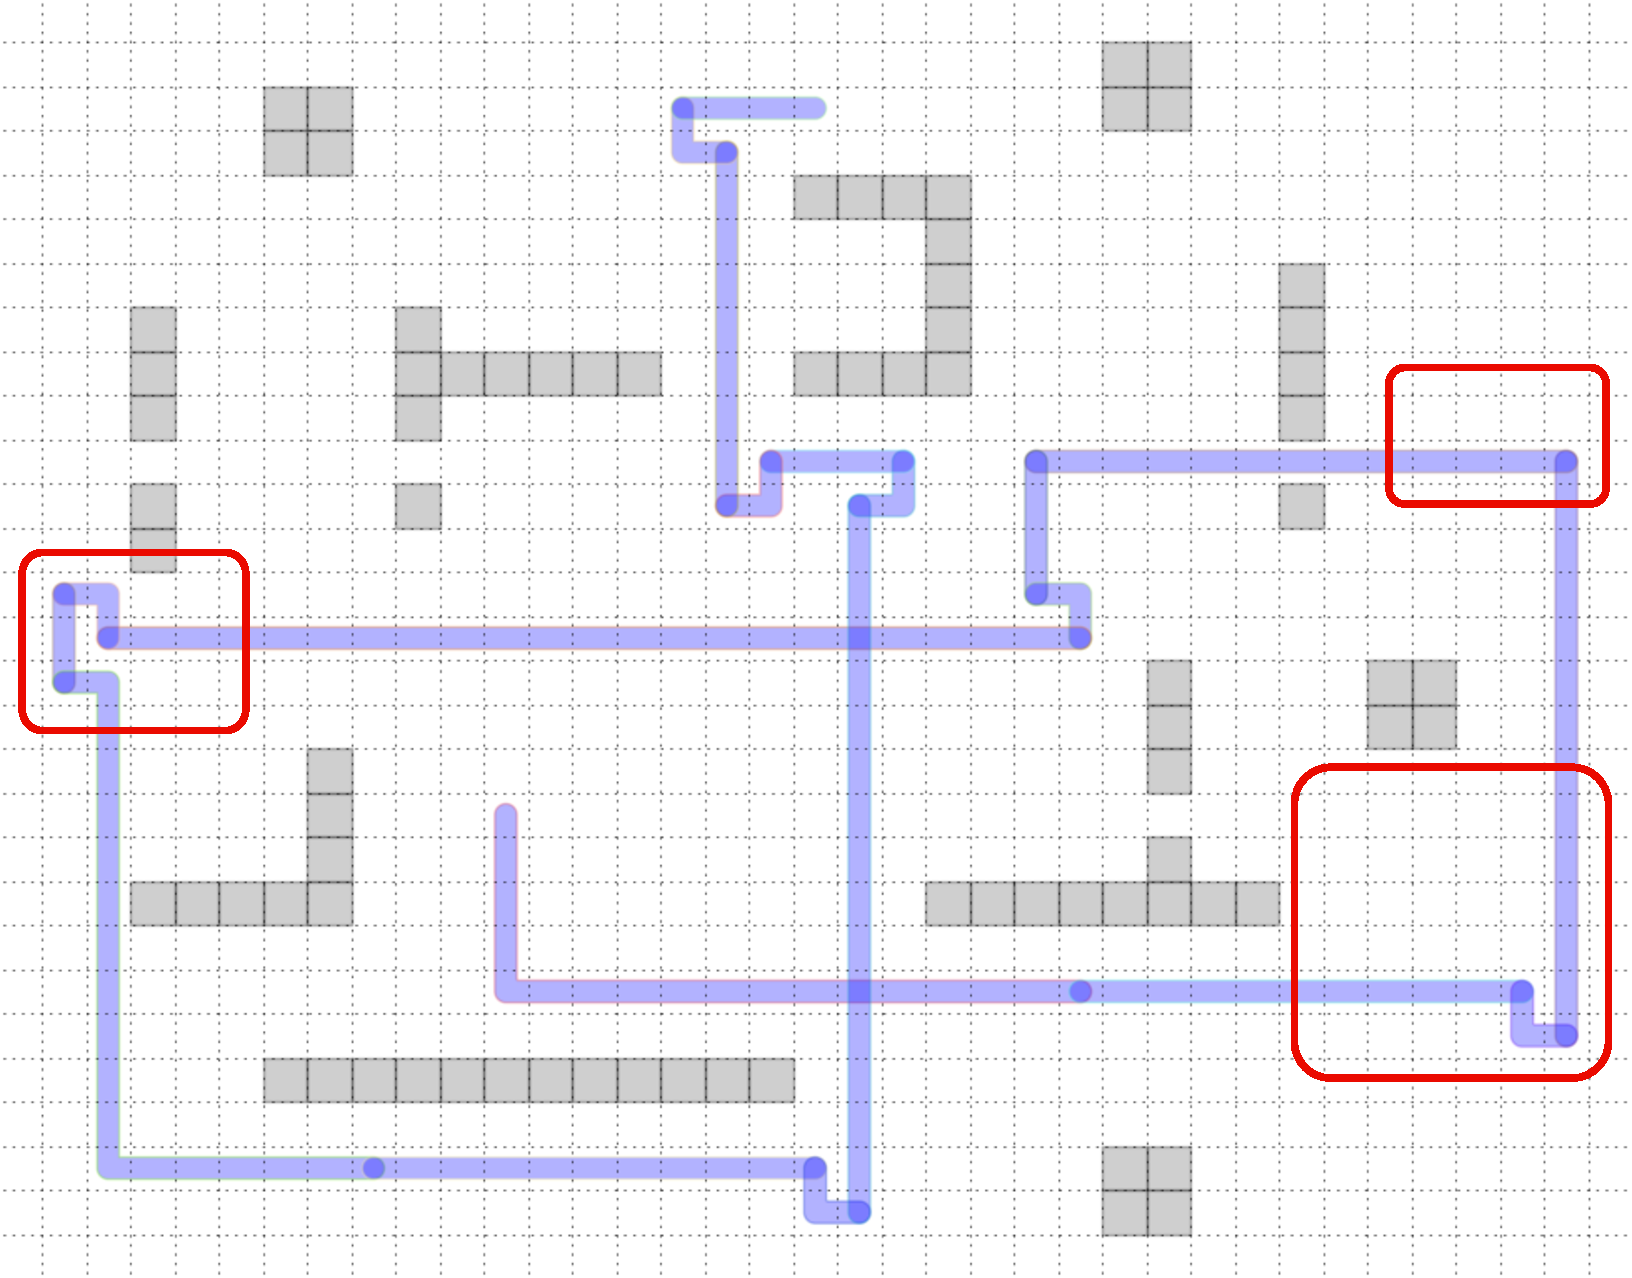
\includegraphics[width=\textwidth]{img/experimentos/ambiente_penalizacao_com.pdf}}
    \caption{Exemplo com a penalização.}
    \label{fig:ambiente_penalizacao_com}
  \end{subfigure}

  \caption[Deslocamento de um agente sem a aplicação da penalização de mudança de direção]{Mapas de deslocamento de um agente demonstrando o transporte de um conjunto de objetos quando é não aplicada a penalização de mudança de direção e o caso onde a penalidade foi utilizada.}
  \label{fig:ambiente_penalizacao_testes}

\end{figure}

Os gráficos a seguir representam o resultado de vários testes realizados, exibindo tanto dados referentes ao deslocamento total dos agentes, quanto ao tempo médio necessário para o planejamento das ações. Foram executados testes tanto aplicando a penalização da mudança de direção quanto sem a mesma. Para uma melhor visualização, foram criados gráficos separando as quantidade de objetos, de 1 a 4 e de 5 a 8, pois a visualização de todos os dados em um só gráfico não permitia uma análise direta devido à escala aplicada nos eixos do gráfico. Cada gráfico exibe em seu eixo horizontal a quantidade de agentes utilizados no experimento, além de representar certas quantidades de objetos sendo transportados por curvas no gráfico.

Os gráficos das figuras \ref{fig:ambiente_penalizacao_deslocamento_sem} e \ref{fig:ambiente_penalizacao_deslocamento_com} demonstram o somatório do deslocamento de todos os agentes, respectivamente os casos onde não foi aplicada a penalização e quando a mesma foi utilizada.
O mesmo pode ser visto nas figuras \ref{fig:ambiente_penalizacao_tempo_sem} e \ref{fig:ambiente_penalizacao_tempo_com}, porém exibindo os dados de tempo de planejamento, no cenário sem e com a penalização.
% Especificamente o gráfico da Figura \ref{fig:ambiente_penalizacao_deslocamento_sem} exibe o caso onde não há penalização, e a Figura \ref{fig:ambiente_penalizacao_deslocamento_penalizado}, o caso com penalização.

% DESLOCAMENTO

\begin{figure}[h]
  \centering
  \setlength{\fboxsep}{0pt}
  \begin{subfigure}[t]{0.49\textwidth}
    \centering
    \fbox{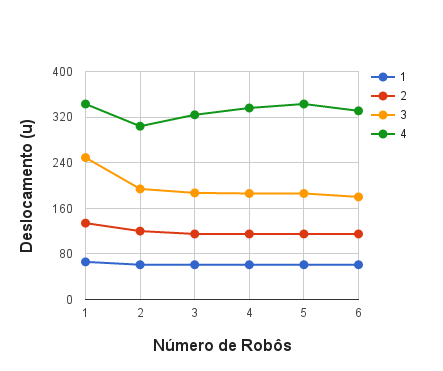
\includegraphics[width=\textwidth]{img/experimentos/penalizacao/penalizado_des_sem_1_4.png}}
    \caption{1 a 4 objetos.}
    % \label{fig:ambiente_penalizacao_deslocamento_normal}
  \end{subfigure}
  \begin{subfigure}[t]{0.49\textwidth}
    \centering
    \fbox{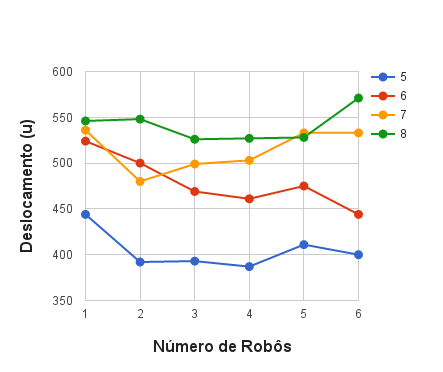
\includegraphics[width=\textwidth]{img/experimentos/penalizacao/penalizado_des_sem_5_8.png}}
    \caption{5 a 8 objetos.}
    % \label{fig:ambiente_penalizacao_deslocamento_penalizado}
  \end{subfigure}
  % Gráficos com o do deslocamento total dos agentes em diferentes configurações de ambientes de teste. Cada curva representa uma certa quantidade de objetos a serem transportados pela equipe, partindo de 1 objeto até 8.
  % Gráficos com o deslocamento total dos agentes, nos casos em que a penalização de mudança de direção não foi aplicada. Cada curva representa uma quantidade distinta de objetos, de 1 a 8.
  \caption[Deslocamento de um agente utilizando a penalização de mudança de direção]{Deslocamento total dos agentes quando não foi aplicada a penalidade de mudança de direção.}
  \label{fig:ambiente_penalizacao_deslocamento_sem}
\end{figure}

\begin{figure}[h]
  \centering
  \setlength{\fboxsep}{0pt}

  \begin{subfigure}[t]{0.49\textwidth}
    \centering
    \fbox{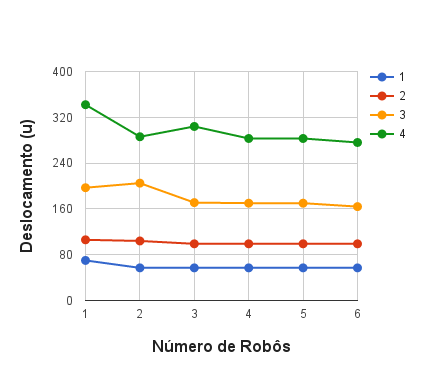
\includegraphics[width=\textwidth]{img/experimentos/penalizacao/penalizado_des_com_1_4.png}}
    \caption{1 a 4 objetos.}
    % \label{fig:ambiente_penalizacao_deslocamento_normal}
  \end{subfigure}
  \begin{subfigure}[t]{0.49\textwidth}
    \centering
    \fbox{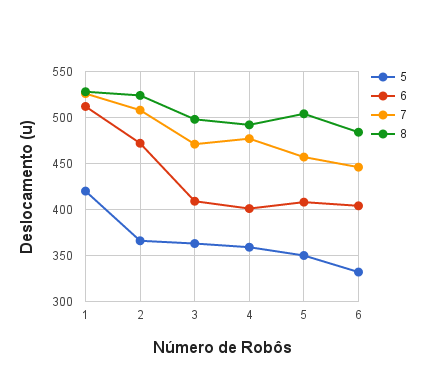
\includegraphics[width=\textwidth]{img/experimentos/penalizacao/penalizado_des_com_5_8.png}}
    \caption{5 a 8 objetos.}
    % \label{fig:ambiente_penalizacao_deslocamento_penalizado}
  \end{subfigure}
  % Gráficos com o do deslocamento total dos agentes em diferentes configurações de ambientes de teste. Cada curva representa uma certa quantidade de objetos a serem transportados pela equipe, partindo de 1 objeto até 8.
  % Gráficos representando o deslocamento total dos agentes durante o transporte com a aplicação da penalização da mudança de direção. Cada curva uma quantidade de objetos transportados, de 1 a 8.
  \caption{Deslocamento total dos agentes com a aplicação da penalidade de mudança de direção.}
  \label{fig:ambiente_penalizacao_deslocamento_com}
\end{figure}

% DESLOCAMENTO

% TEMPO

\begin{figure}[h]
  \centering
  \setlength{\fboxsep}{0pt}

  \begin{subfigure}[t]{0.49\textwidth}
    \centering
    \fbox{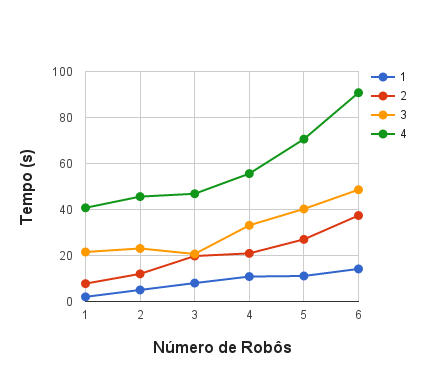
\includegraphics[width=\textwidth]{img/experimentos/penalizacao/penalizado_tem_sem_1_4.png}}
    \caption{1 a 4 objetos.}
    % \label{fig:ambiente_penalizacao_tempo_normal}
  \end{subfigure}
  \begin{subfigure}[t]{0.49\textwidth}
    \centering
    \fbox{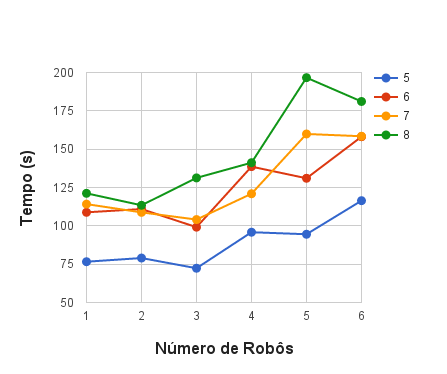
\includegraphics[width=\textwidth]{img/experimentos/penalizacao/penalizado_tem_sem_5_8.png}}
    \caption{5 a 8 objetos.}
    % \label{fig:ambiente_penalizacao_tempo_penalizado}
  \end{subfigure}
  % Gráficos representativos do tempo de planejamento dos agentes em cenários com diferentes quantidades de objetos e robôs. Cada curva representa uma certa quantidade de objetos.
  \caption{Tempo de planejamento dos agentes sem a aplicação da penalidade de mudança na direção.}
  \label{fig:ambiente_penalizacao_tempo_sem}
\end{figure}

\begin{figure}[h]
  \centering
  \setlength{\fboxsep}{0pt}

  \begin{subfigure}[t]{0.49\textwidth}
    \centering
    \fbox{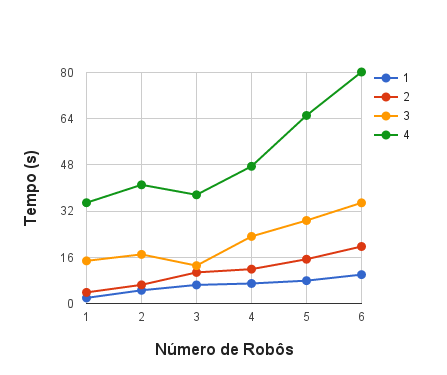
\includegraphics[width=\textwidth]{img/experimentos/penalizacao/penalizado_tem_com_1_4.png}}
    \caption{1 a 4 objetos.}
    % \label{fig:ambiente_penalizacao_tempo_normal}
  \end{subfigure}
  \begin{subfigure}[t]{0.49\textwidth}
    \centering
    \fbox{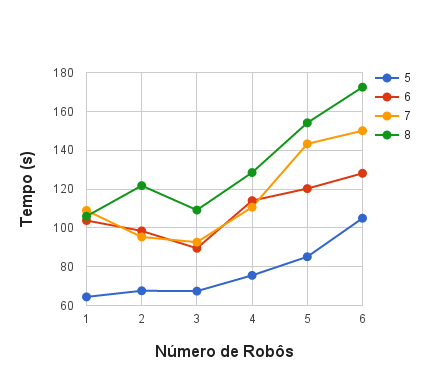
\includegraphics[width=\textwidth]{img/experimentos/penalizacao/penalizado_tem_com_5_8.png}}
    \caption{5 a 8 objetos.}
    % \label{fig:ambiente_penalizacao_tempo_penalizado}
  \end{subfigure}
  % Gráficos representativos do tempo de planejamento dos agentes em cenários com diferentes quantidades de objetos e robôs. Cada curva representa uma certa quantidade de objetos.
  \caption{Tempo de planejamento dos agentes com a aplicação da penalidade de mudança na direção.}
  \label{fig:ambiente_penalizacao_tempo_com}
\end{figure}

% TEMPO

Ao analisar os gráficos de deslocamento, é possível notar que nos casos em que não há a penalização da mudança de direção, o sistema não se beneficia tanto da quantidade de agente, que contrariamente ao esperado, aumenta a distância percorrida quando a equipe aumenta de tamanho.
Comportamento este que não é observado quando é a aplicada a penalização, em que a tendência do sistema é necessitar de uma menor quantidade total de deslocamento para realizar o transporte dos objetos.
A diminuição nos trajetos era esperada, considerando que uma maior quantidade de agentes garante uma maior diversidade de opções para transportar um determinado objeto, criando mais chances de existirem robôs com planos melhores, contribuindo para minimizar a movimentação geral.

Apesar da diminuição na movimentação dos agentes com a penalização, em alguns casos, é notado que o aumento da quantidade de agentes, mesmo que sutil, faz com que os agentes andem mais que nos casos com uma menor equipe, como na situação do transporte de 8 objetos por 4 e 5 agentes.
Isso é explicado pelo fato do algoritmo de alocação de tarefas (Seção \ref{sec:aloca_o_de_tarefas}) sempre alocar tarefas para todos os agentes, mesmo que a melhor configuração fosse deixar um determinado robô sem nenhuma tarefa, afetando assim o deslocamento total dos agentes.
Mesmo com este acréscimo, deve ser lembrado que com mais agentes, executando mais tarefas ao mesmo tempo, o tempo de execução total da tarefa reduzirá.

Em relação ao tempo de planejamento, um efeito contrário é observado. Seja com o aumento no número de objetos ou no número de agentes, o sistema tende a consumir mais tempo para planejar todas as rotas necessárias para o transporte.
O aumento no número de objetos faz com que os agentes tenham mais opções de planos a executar, já o aumento no número de agentes aumenta a quantidade de possíveis robôs para executar o transporte de um objeto, além de uma necessidade maior de tempo para que toda a equipe entre em acordo sobre quais tarefas executar.
Mesmo com este comportamento, observa-se nos gráficos onde há a aplicação da penalidade, o tempo necessário para o planejamento é sempre menor ou bastante aproximado dos casos em que não é aplicada, demonstrando como esta estratégia contribui para o melhoramento da performance do sistema.

% Ao analisar os gráficos de deslocamento, dois pontos podem ser notados: (i) conforme o número de agentes na equipe aumenta, a distância total percorrida decai, isto porque existe uma maior chance de haver um agente próximo ao um determinado objeto, retirando a responsabilidade de outro robô distante do mesmo e assim minimizando todos os planos; e (ii) na presença de penalização é perceptível que os planos em sua maioria são minimizados, isto é explicado quando o agente não necessita empurrar o objeto de diferentes posições, criando menos planos de preparação e consequentemente, reduzindo o espaço de deslocamento.

% Apesar disso, um efeito contrário é observado na dimensão de tempo do planejamento. Quando existe uma equipe maior de agentes e maior número de objetos, maior é o tempo necessário para que todos planejem e entrem em acordo sobre as tarefas a serem realizadas.

Estes fatores são interessantes de serem estudados pois ocasionam um \emph{trade-off} entre a quantidade de robôs a ser utilizada, o tempo de planejamento e o ganho em deslocamento total.
Encontrar a melhor combinação destes valores não foi objetivo deste trabalho, mas sim demonstrar que cada uma destas variáveis influencia diretamente na performance total do sistema.

% subsection deslocamento_e_templo_de_planejamento_dos_agentes (end)

\subsection{Função de Utilidade} % (fold)
\label{sub:fun_o_de_utilidade}

Durante o desenvolvimento do método, chegou-se à conclusão que seria possível criar um sistema no qual fosse possível configurar os algoritmos de planejamento de modo a atender diferentes demandas, criando planos que fossem ou mais rápidos de serem executados, ou mesmo com um menor custo energético para realização.

Esta configuração é possível através de um artifício na heurística utilizada no algoritmo modificado A* utilizado nas etapas de criação dos planos de movimentação.
A função heurística descrita na Seção \ref{sub:fun_o_de_avalia_o} exerce sua influência para modificar o plano.

Neste sentido, foram realizados experimentos em um mapa simples, como o demonstrado a seguir na Figura \ref{fig:utility_function_graph}, modificando as constantes de ponderação em cada dimensão analisada, tempo e energia. A Tabela \ref{table:utility_function_graph} expõe os pesos utilizado em cada experimento.

\begin{table}
    \centering
    \caption[Tabela com as variações nos pesos da função de utilidade]{Tabela com as variações nos pesos utilizados para realização de testes aplicados na função de utilidade durante a fase de planejamento dos objetos.}
    \label{table:utility_function_graph}
    \begin{tabular}{|c|c|c|}
    \hline
    Experimento & Tempo & Energia \\ \hline
    1        & 1     & 0       \\ \hline
    2        & 0     & 1       \\ \hline
    3        & 0.5   & 0.5     \\ \hline
    \end{tabular}
\end{table}

Um fato importante de ser mencionado é que estes experimentos, apesar de serem reflexo da influência da função de utilidade, só possuem sentido levando em consideração as características dos agentes utilizados durante o planejamento.
Estes parâmetros são utilizados durantes os cálculos para decidir a utilidade de certa ação de movimento realizada por cada tipo de agente, e assim, decidir o melhor caminho que atenda às configurações previamente estabelecidas pelas constantes de ponderação.

Os experimentos ilustrados nos mapas da Figura \ref{fig:utility_function_graph}, utilizam dois tipos de agentes, um terrestre e outro aéreo. Para averiguar as características dos mesmo, foram realizados dois tipos de testes: (i) a velocidade média de deslocamento entre dois pontos fixos do ambiente, considerando somente a movimentação em linha reta, e (ii) o tempo médio de duração da bateria em uso contínuo.
Uma vez realizados estas provas, a tabela \ref{table:caracteristicas} apresenta os valores estimados para cada tipo de agente.
Estes dados são demonstrados de forma unitária, ou seja, o agente com melhor performance em uma determinada característica possui valor 1, e o outro agente possui um valor determinado em quantas vezes o mesmo é pior naquela propriedade.
Estes dados não são fixos ou finais, pois estão diretamente relacionados ao tipos de agentes utilizados durantes os testes, podendo haver uma grande diferença se outras plataformas robótica fossem utilizadas durante as provas.

\begin{table}
    \centering
    \caption[Dados referente às características dos tipos de agentes]{Dados referente às características dos tipos de agentes utilizados durante os experimentos da função de utilidade.}
    \label{table:caracteristicas}
    \begin{tabular}{|c|c|c|}
    \hline
    Tipo      & Energia & Tempo \\ \hline
    Terrestre & 1       & 8     \\ \hline
    Aéreo     & 12      & 1     \\ \hline
    \end{tabular}
\end{table}

\begin{figure}[htpb]
  \centering
  \setlength{\fboxsep}{0pt}

  \begin{subfigure}[t]{0.315\textwidth}
    \centering
    \fbox{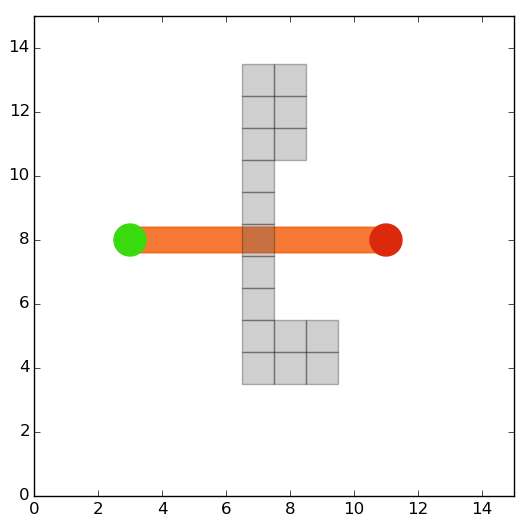
\includegraphics[width=\textwidth]{img/experimentos/utility_func_time.png}}
    \caption{Experimento 1}
    % Plano do objeto favorecendo o tempo de execução. Variação 1.
    \label{fig:utility_function_time}
  \end{subfigure}
  \hspace{0.1cm}
  \begin{subfigure}[t]{0.315\textwidth}
    \centering
    \fbox{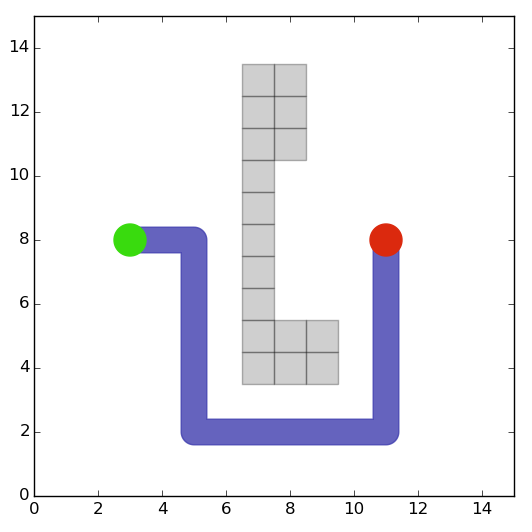
\includegraphics[width=\textwidth]{img/experimentos/utility_func_energy.png}}
    \caption{Experimento 2}
    % Plano do objeto priorizando o baixo custo energético. Variação 2.
    \label{fig:utility_function_energy}
  \end{subfigure}
  \hspace{0.1cm}
  \begin{subfigure}[t]{0.315\textwidth}
    \centering
    \fbox{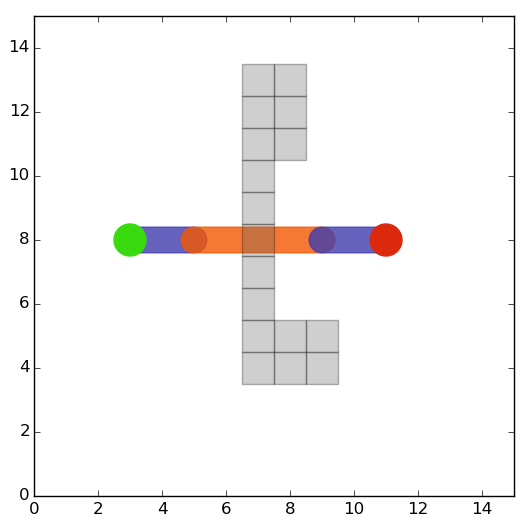
\includegraphics[width=\textwidth]{img/experimentos/utility_func_mid.png}}
    \caption{Experimento 3}
    % Plano do objeto realizando uma mediação entre tempo e energia. Variação 3.
    \label{fig:utility_function_mid}
  \end{subfigure}

  \caption[Exemplos de planos de movimentação de um objeto com diferentes pesos na função de utilidade]{Exemplos de planos de movimentação de um objeto mediante a troca das constantes de ponderação na função de utilidade utilizada como heurística do planejador. O caminho demarcado em laranja representa um trajeto aéreo, enquanto o lilás é terrestre.}
  \label{fig:utility_function_graph}

\end{figure}

Mediante os dados expostos, é possível observar como a mudança nos pesos da função de utilidade é capaz de atuar sobre os planos criados, tornando o método apresentado flexível, passível de ser configurado para atender a diferentes necessidades.

% subsection fun_o_de_utilidade (end)

\subsection{Sequenciamento do Transporte} % (fold)
\label{sub:tipo_de_transporte}

Um importante fator durante a ação de transporte de objetos é a escolha da sequência na qual estes objetos serão manipulados, pois, uma ordenação mal determinada pode levar os agentes a transcorrer grandes distâncias para realizar o deslocamento.

Neste experimento serão realizados experimentos comparando dois tipos de transporte: (i) sequencial -- na qual os objetos são manipulados em uma ordem pré-definida, não avaliando qualquer custo excessivo associado ao deslocamento dos agentes, e (ii) oportunista -- onde é avaliado o melhor objeto a ser transportado em um determinado momento baseado na localização do agente, procurando sempre minimizar a distância percorrida.

De forma demonstrativa, são exibidos na Figura \ref{fig:figure_simple_smart} dois gráficos com o deslocamento de um agente realizando o transporte de 3 objetos, onde são destacadas as áreas de maior discrepância entre os resultados do tipo de transporte.
O mapa utilizado durante este experimento é similar ao da Figura \ref{fig:cenario_sequencial_oportunista}.
Como pode ser observado, durante o transporte sequencial o agente realiza planos mais longos, pois esta métrica (tamanho do plano) não é levada em consideração durante a escolha do objeto, em comparação ao transporte oportunista, que sempre visa o objeto com melhor custo, este apresenta um comportamento com menor distâncial total percorrida nos planos.

O mapa apresentado na Figura \ref{fig:cenario_sequencial_oportunista} ilustra o ambiente no qual os demais experimentos foram realizados, nos quais também um agente foi utilizado, o que proporciona uma melhor visualização do seu deslocamento referente à sequência do transporte.

\begin{figure}[h]
  \centering
  \setlength{\fboxsep}{0pt}

  \begin{subfigure}[t]{0.45\textwidth}
    \centering
    \fbox{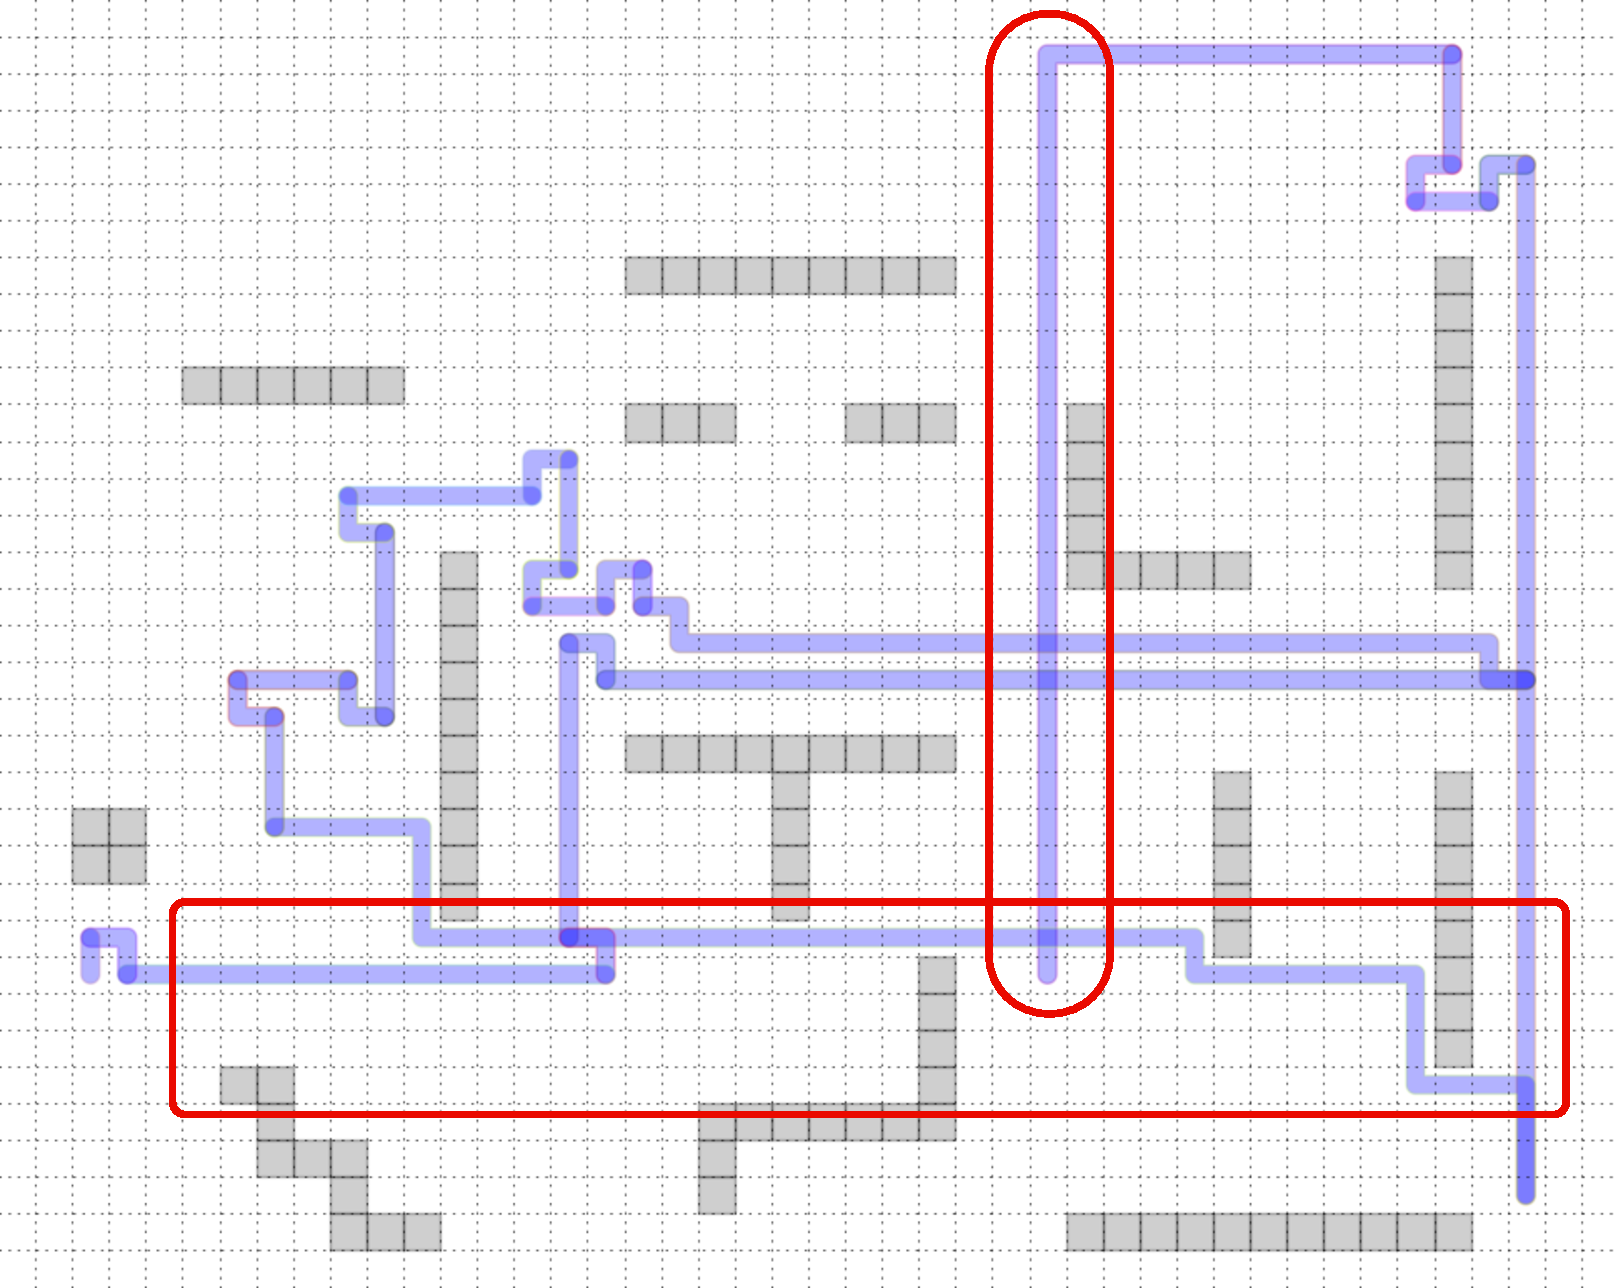
\includegraphics[width=\textwidth]{img/experimentos/figure_simple.pdf}}
    \caption{Transporte sequencial}
    \label{fig:figure_simple}
  \end{subfigure}
  \hspace{0.2cm}
  \begin{subfigure}[t]{0.45\textwidth}
    \centering
    \fbox{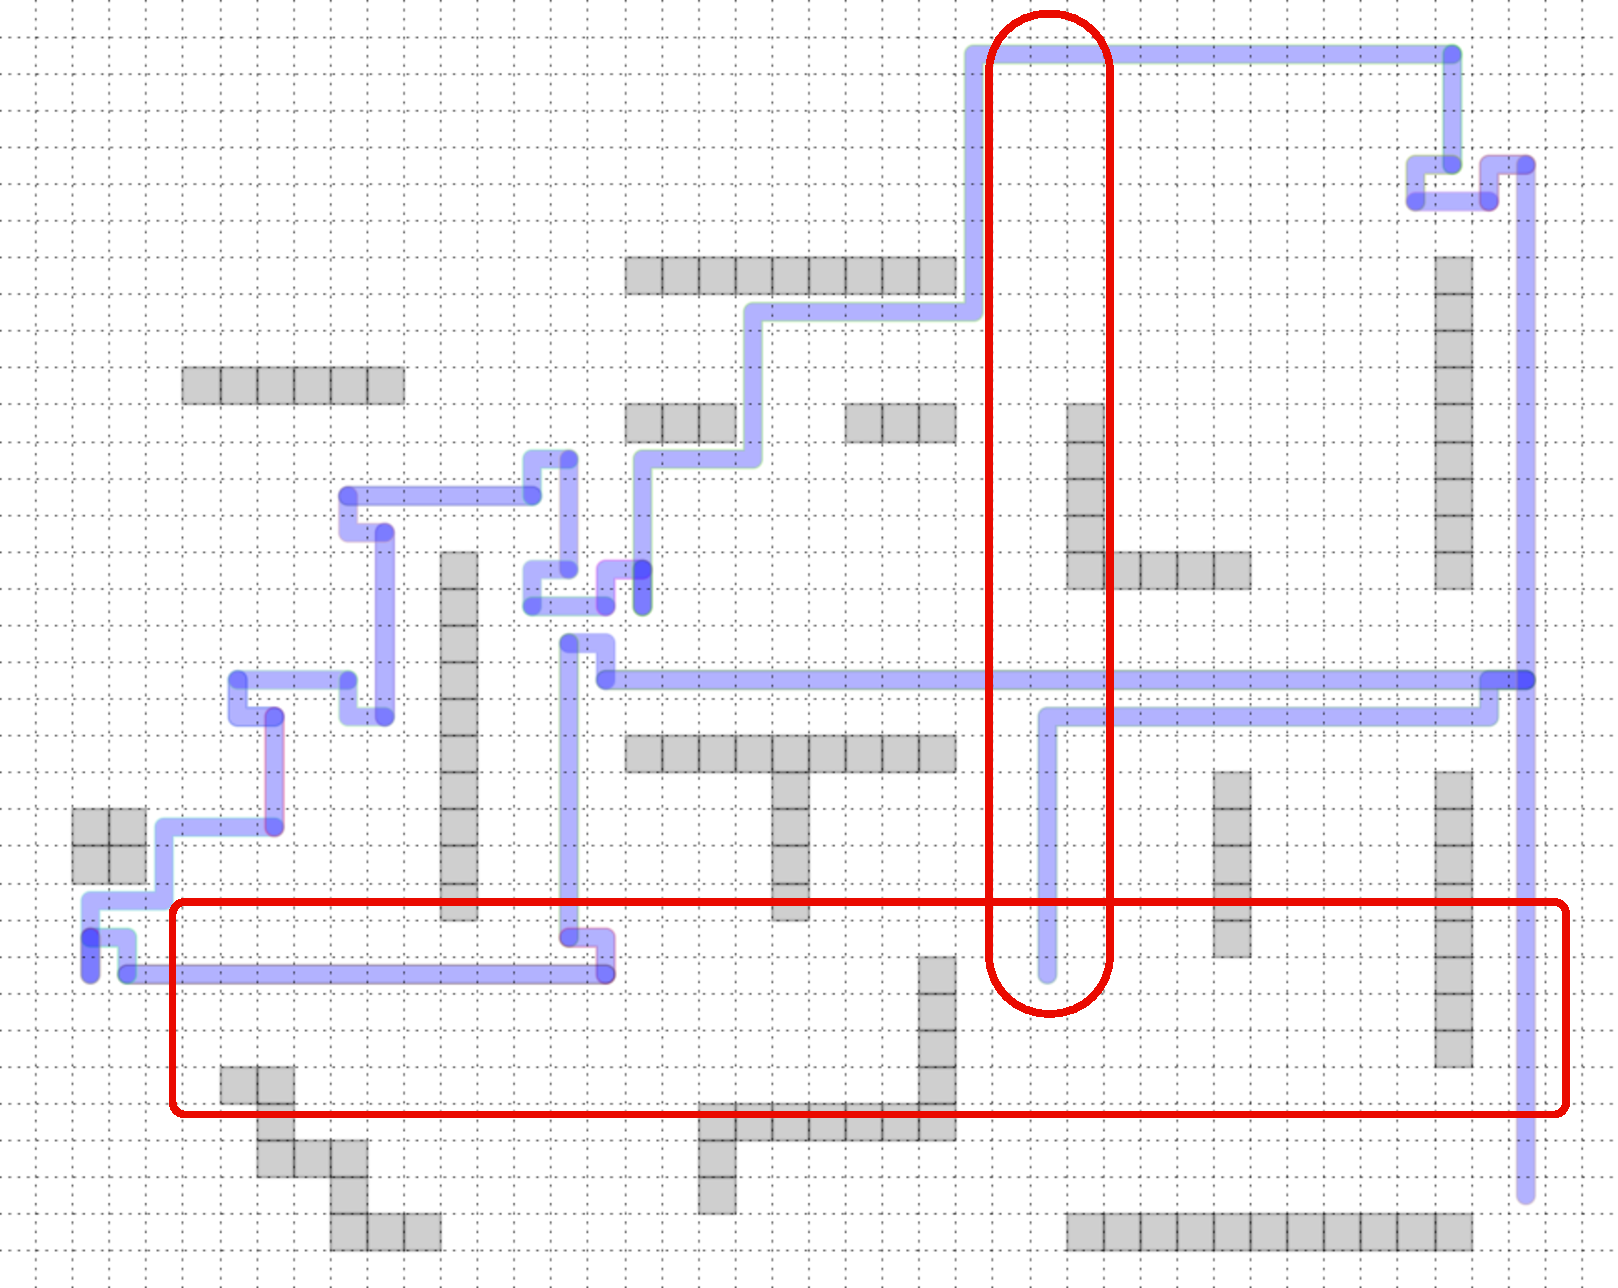
\includegraphics[width=\textwidth]{img/experimentos/figure_smart.pdf}}
    \caption{Transporte oportunista}
    \label{fig:figure_smart}
  \end{subfigure}

  \caption[Resultado do transporte de 3 objetos por um agente]{Resultado do transporte de 5 objetos por um agente utilizando o método sequencial e o oportunista.}
  \label{fig:figure_simple_smart}

\end{figure}

\begin{figure}[h]
  \centering
  \setlength{\fboxsep}{0pt}
  \fbox{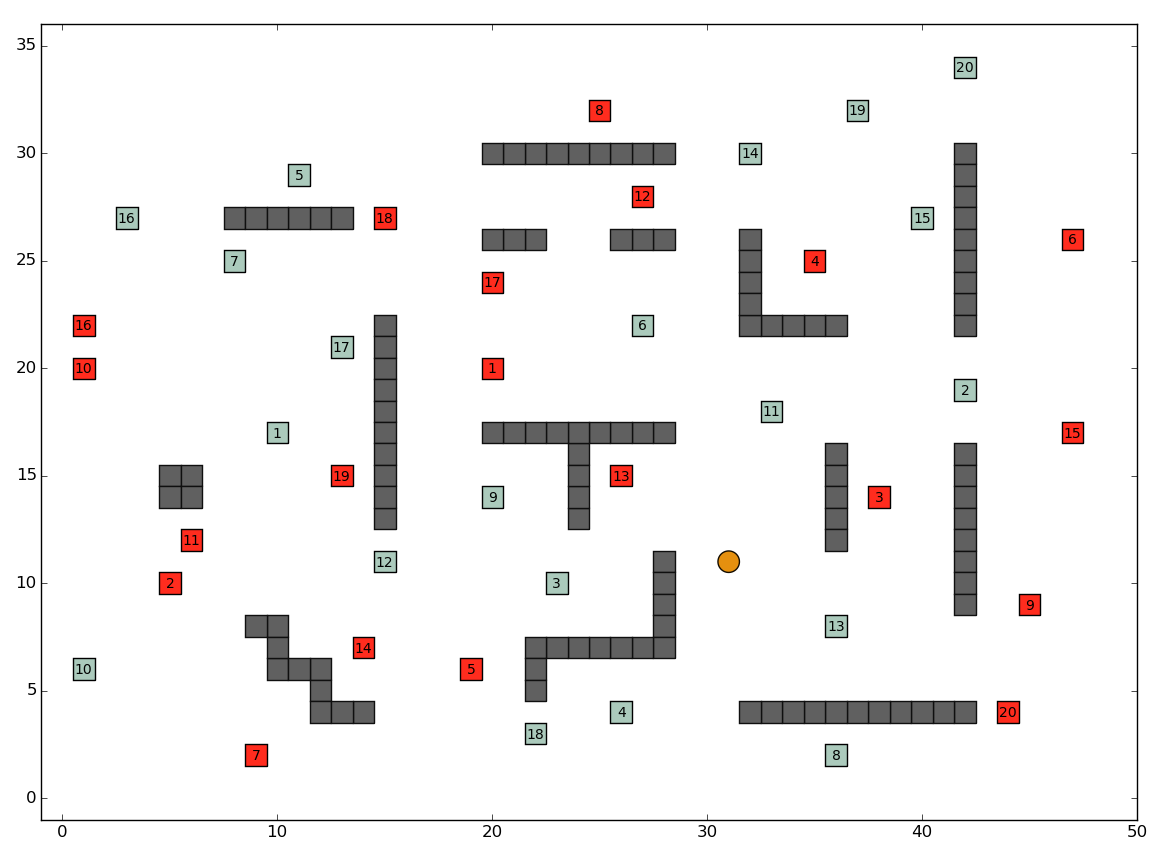
\includegraphics[width=0.5\textwidth]{img/experimentos/mapa_sequencial_oportunista.png}}
  \caption[Mapa utilizado nos testes sequencial e oportunista]{Mapa utilizado para avaliar a diferenciação entre os tipos de atitudes no transporte, sequencial e oportunista.}
  \label{fig:cenario_sequencial_oportunista}
\end{figure}

\begin{figure}[h]
  \centering
  \setlength{\fboxsep}{0pt}
  \fbox{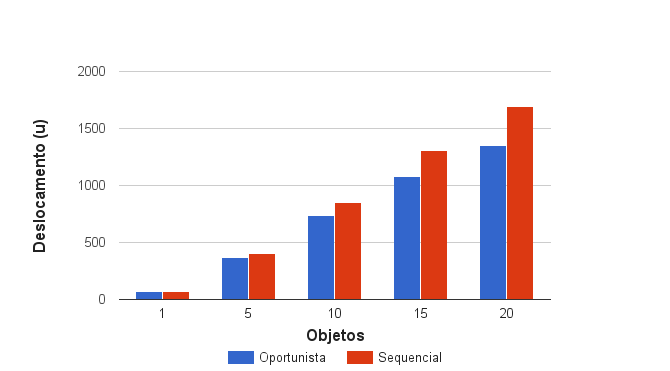
\includegraphics[width=0.8\textwidth]{img/experimentos/sequencial_oportunista_deslocamento.png}}
  \caption[Deslocamento do robô mediante nos transportes sequencial e oportunista]{Deslocamento do robô mediante a adição de objetos utilizando dois tipos de transporte, sequencial e oportunista.}
  \label{fig:cenario_sequencial_oportunista_deslocamento}
\end{figure}

\begin{figure}[h]
  \centering
  \setlength{\fboxsep}{0pt}
  \fbox{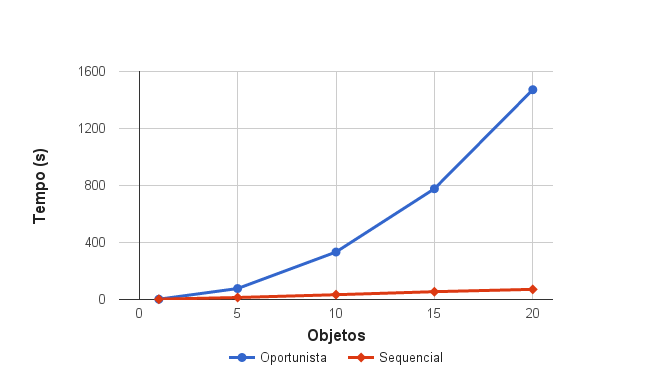
\includegraphics[width=0.8\textwidth]{img/experimentos/sequencial_oportunista_tempo.png}}
  \caption[Tempo de planejamento do agente nos transporte sequencial e oportunista]{Tempo de planejamento do agente nas duas técnicas de transporte, sequencial e oportunista.}
  \label{fig:cenario_sequencial_oportunista_tempo}
\end{figure}

A Figura \ref{fig:cenario_sequencial_oportunista_deslocamento} demonstra um gráfico comparativo entre as distâncias percorridas pelo agente quando o número de objetos a ser transportado aumenta. Mesmo que os planos se tornem mais longos com a adição de objetos, que é um fato esperado, é possível perceber que o método oportunista faz um melhor uso da posição do robô, proporcionando uma menor travessia total e assim economizando tanto tempo como energia, pois estes custos estão diretamente relacionados ao tamanho do plano executado.

Apesar da vantagem apresentada, como é demonstrado no gráfico da Figura \ref{fig:cenario_sequencial_oportunista_tempo}, o tempo necessário de planejamento no caso oportunista apresenta um comportamento de crescimento muito superior à técnica sequencial.
Este desempenho é justificado ao considerar que o agente deve decidir qual o melhor objeto a transportar, e para tal, deve considerar planos de transporte para todos os objetos ainda não transportados, gerando uma maior demanda de tempo nesta etapa, diferente da técnica sequencial, na qual somente o objeto atualmente sendo manipulado é tido como base pra realização do planejamento.

Porém, é interessante ressaltar que, apesar do grande gasto de tempo durante o planejamento, este não afeta drasticamente o gasto energético do agente, pois o mesmo não está em movimentação, o que justifica o uso da técnica oportunista, considerando que o ganho proporcionado por um menor plano é superior ao ganho quando o planejamento é executado rapidamente.

\section{Ambiente Simulado} % (fold)
\label{sub:ambiente_simulado}

Para realização dos testes simulados, foi utilizado o \emph{Robot Operating System (ROS)}\footnote{www.ros.org}, que é um conjunto bibliotecas para desenvolvimento de plataformas autônomas largamente utilizado tanto em pesquisas quanto em aplicações comerciais. Especificamente a versão \emph{Indigo} foi utilizada na implementação.
Este sistema abstrai as camadas de envio e recebimento de dados, provendo acesso aos sensores e atuadores de diversas plataformas robóticas.

Os algoritmos desenvolvidos foram testados no ambiente de simulação \emph{Gazebo}\footnote{http://gazebosim.org/}. O mesmo já possui integração direta com o \emph{ROS}, capaz de simular a dinâmica entre corpos virtuais utilizando diferentes motores de física (\emph{ODE}, \emph{Bullet}, \emph{Simbody}, \emph{DART}), além de implementar uma diversidade de sensores (câmeras RGB-D, laser, torque) e possuir vários modelos pré-existentes para criação de ambientes realísticos, tanto de robôs, mas também inclui ferramentas, casas, véículos, dentre outros.

Para uma demonstração da técnica apresentada por este trabalho, serão documentados dois experimentos simulados, visando exemplificar o processo de coordenação entre diferentes agentes. Serão apresentados dois casos do transporte de um objeto: (i) dois agentes terrestres e (ii) um agente terrestre e outro aéreo.

A Figura \ref{fig:maps} demonstra os ambientes de trabalho construídos para a simulação. Neles é possível observar a disposição do objeto a ser transportado, bem como dos agentes e obstáculos.

\begin{figure}[h]
  \centering
  \setlength{\fboxsep}{0pt}

  \begin{subfigure}[t]{0.45\textwidth}
    \centering
    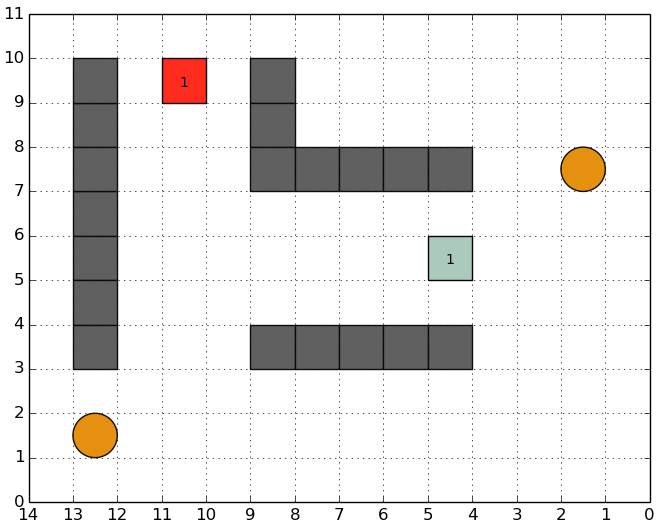
\includegraphics[width=\textwidth]{img/experimentos/sim_map1.png}
    \caption{Dois agentes terrestres.}
  \end{subfigure}
  \hspace{0.2cm}
  \begin{subfigure}[t]{0.45\textwidth}
    \centering
    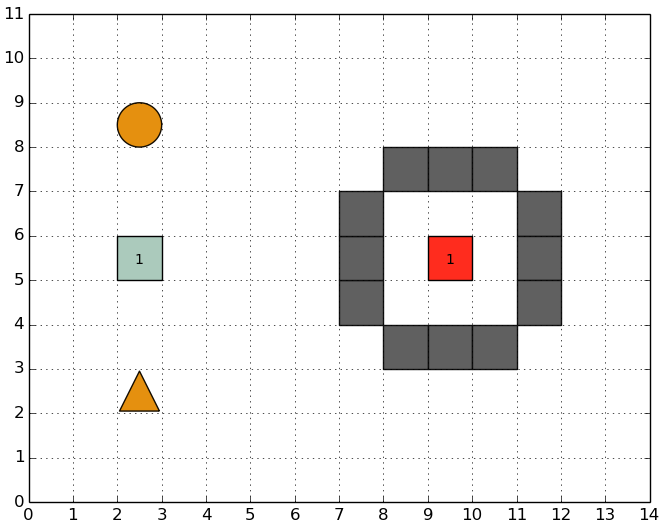
\includegraphics[width=\textwidth]{img/experimentos/sim_map2.png}
    \caption{Um agente terrestre e outro aéreo.}
  \end{subfigure}

  \caption{Ambientes de trabalho utilizados durante os experimentos simulados.}
  \label{fig:maps}

\end{figure}

A Figura \ref{fig:sim_ground} ilustra o transporte de um objeto por uma equipe de dois agentes terrestres. Os agentes representados são da plataforma \emph{iRobot Create}, robô diferencial com dimensões de 33cm de diâmetro e 12cm de altura, capazes de executar somente a ação de \emph{PUSH} no objeto.
Cada sub-figura ilustra um determinado estado do sistema com seu respectivo tempo de ocorrência.

\begin{figure}[ht!]
  \centering
  \setlength{\fboxsep}{0pt}

  \begin{subfigure}[t]{0.45\textwidth}
    \centering
    \fbox{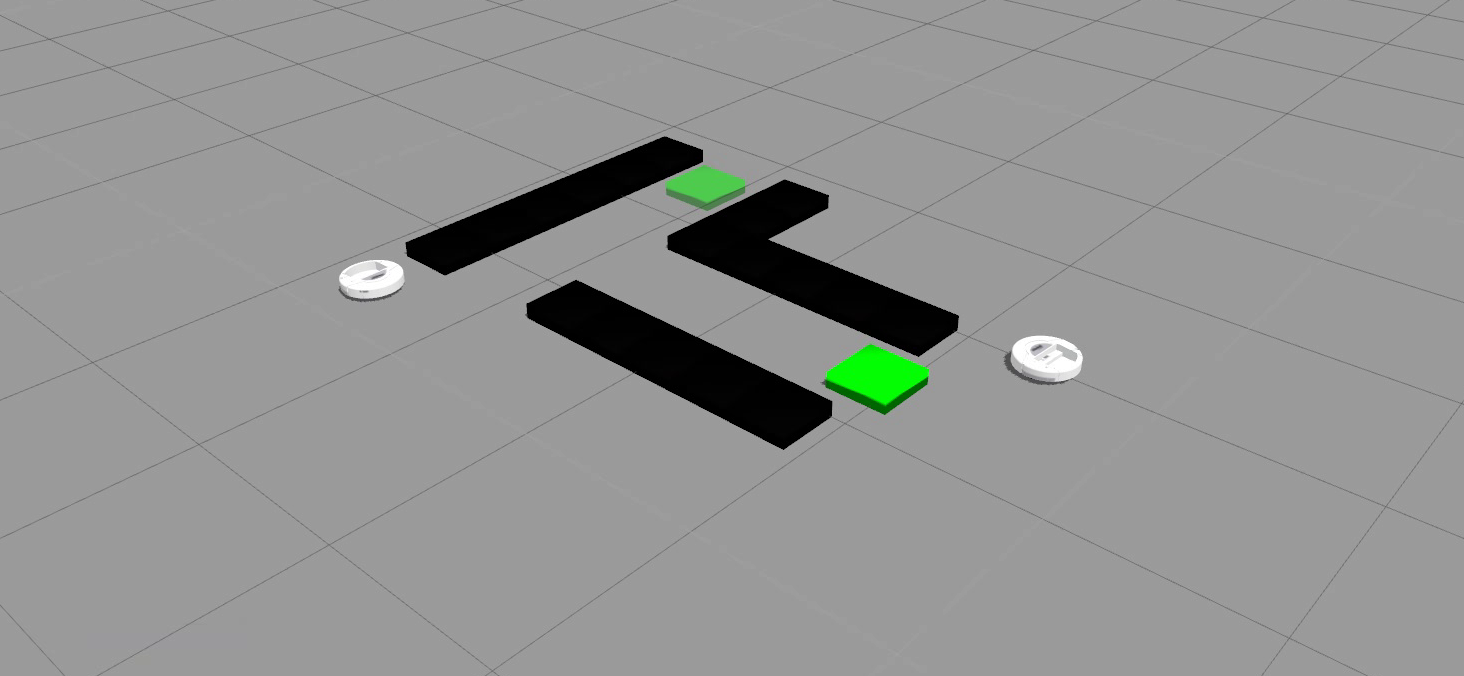
\includegraphics[width=\textwidth]{img/experimentos/sim_001.png}}
    \caption{t=1s}
    \label{fig:sim_1}
  \end{subfigure}
  \hspace{0.2cm}
  \begin{subfigure}[t]{0.45\textwidth}
    \centering
    \fbox{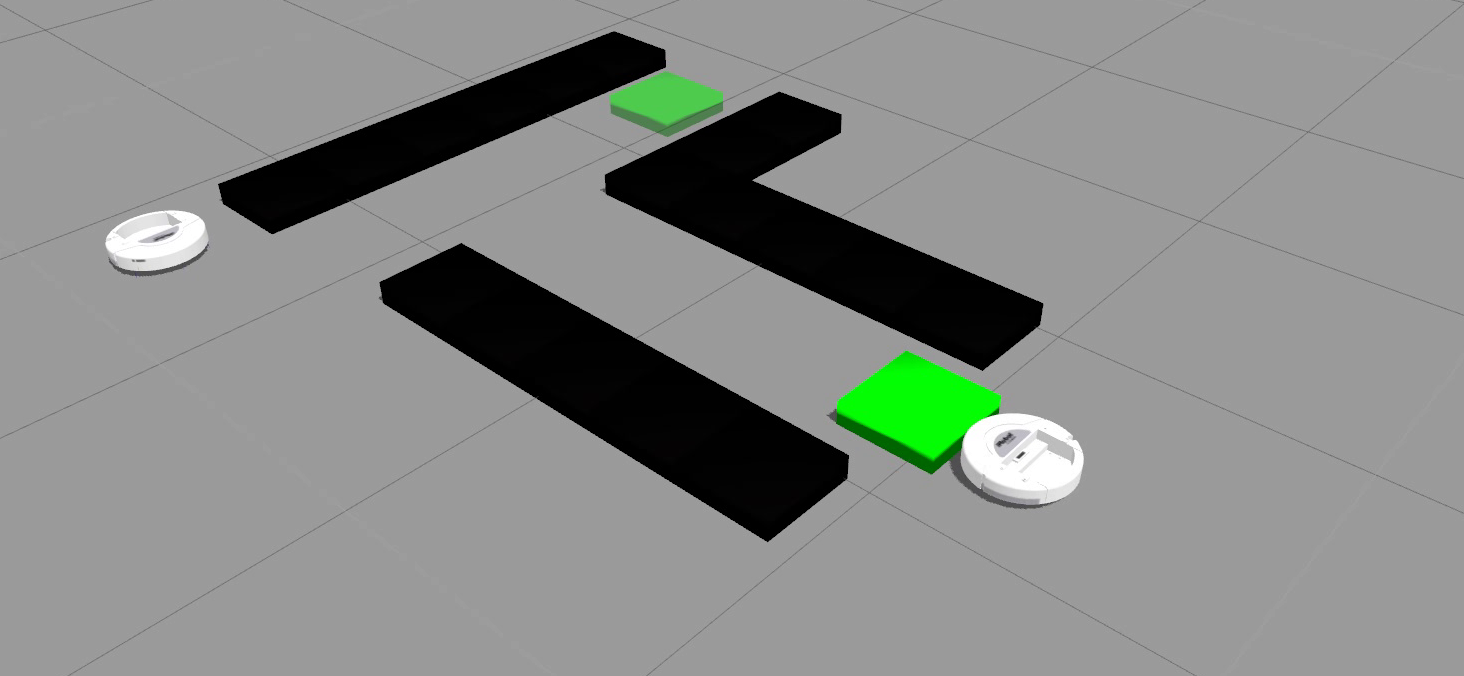
\includegraphics[width=\textwidth]{img/experimentos/sim_044.png}}
    \caption{t=44s}
    \label{fig:sim_44}
  \end{subfigure}

  \begin{subfigure}[t]{0.45\textwidth}
    \centering
    \fbox{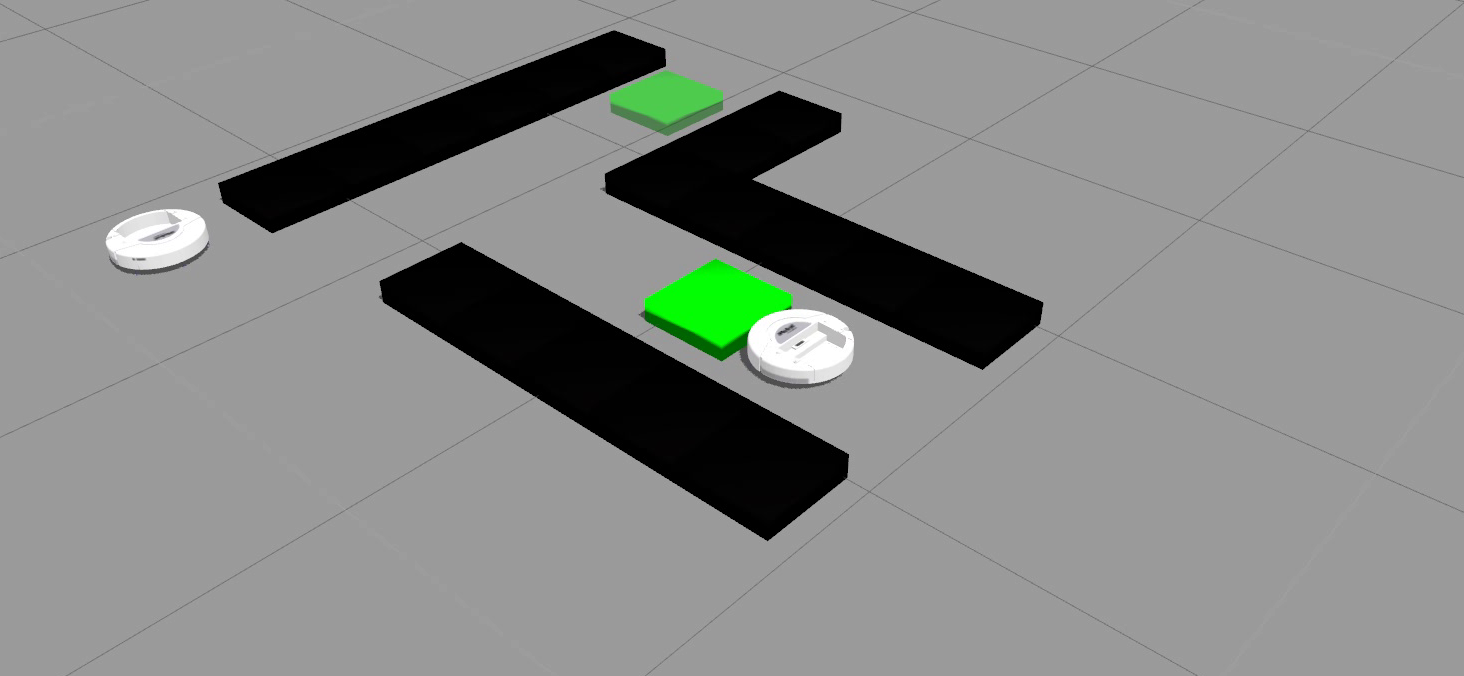
\includegraphics[width=\textwidth]{img/experimentos/sim_078.png}}
    \caption{t=78s}
    \label{fig:sim_78}
  \end{subfigure}
  \hspace{0.2cm}
  \begin{subfigure}[t]{0.45\textwidth}
    \centering
    \fbox{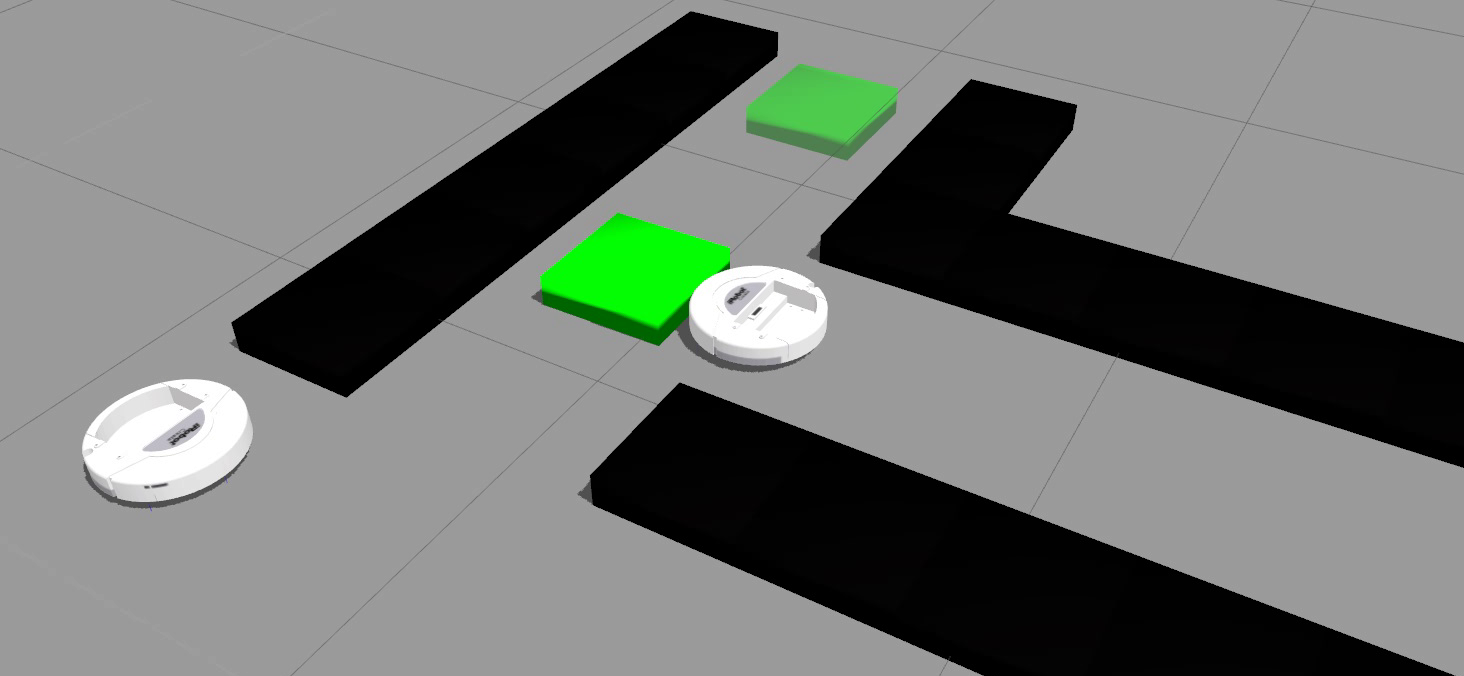
\includegraphics[width=\textwidth]{img/experimentos/sim_139.png}}
    \caption{t=139s}
    \label{fig:sim_139}
  \end{subfigure}

  \begin{subfigure}[t]{0.45\textwidth}
    \centering
    \fbox{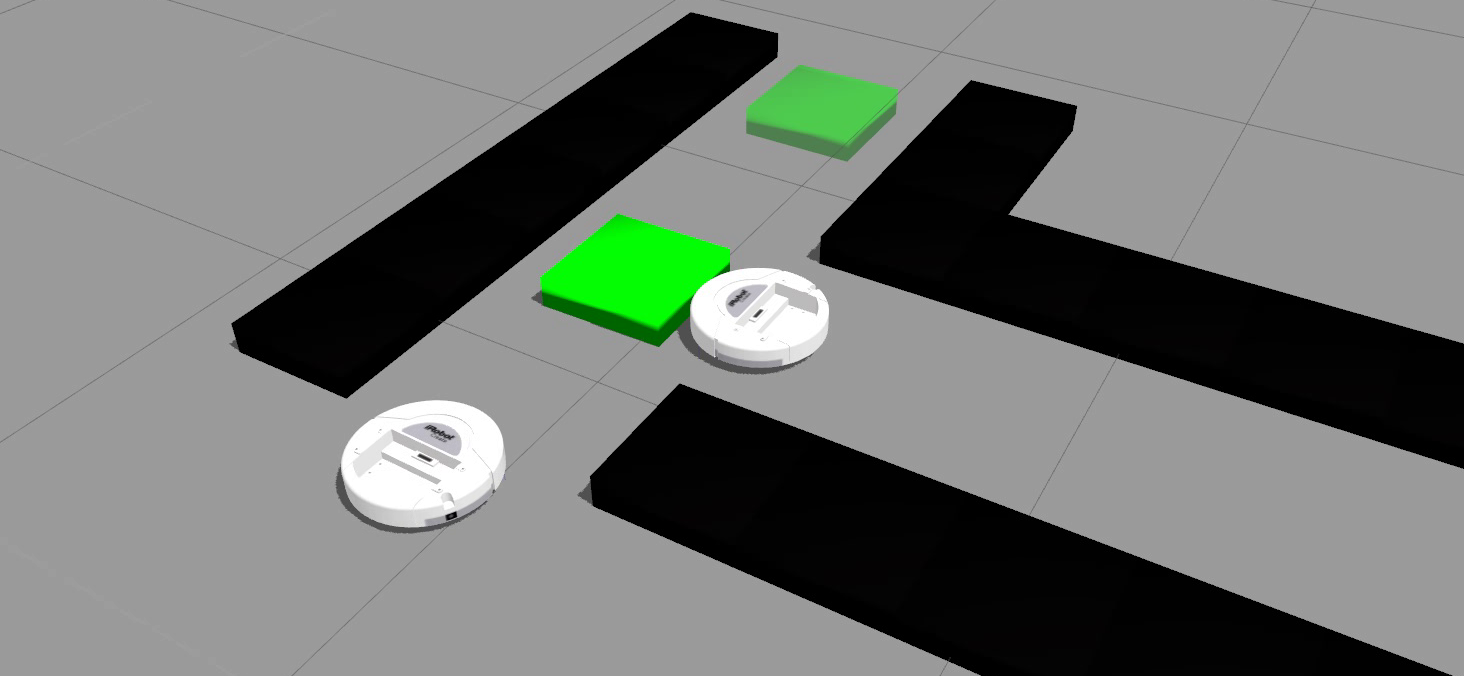
\includegraphics[width=\textwidth]{img/experimentos/sim_180.png}}
    \caption{t=180s}
    \label{fig:sim_180}
  \end{subfigure}
  \hspace{0.2cm}
  \begin{subfigure}[t]{0.45\textwidth}
    \centering
    \fbox{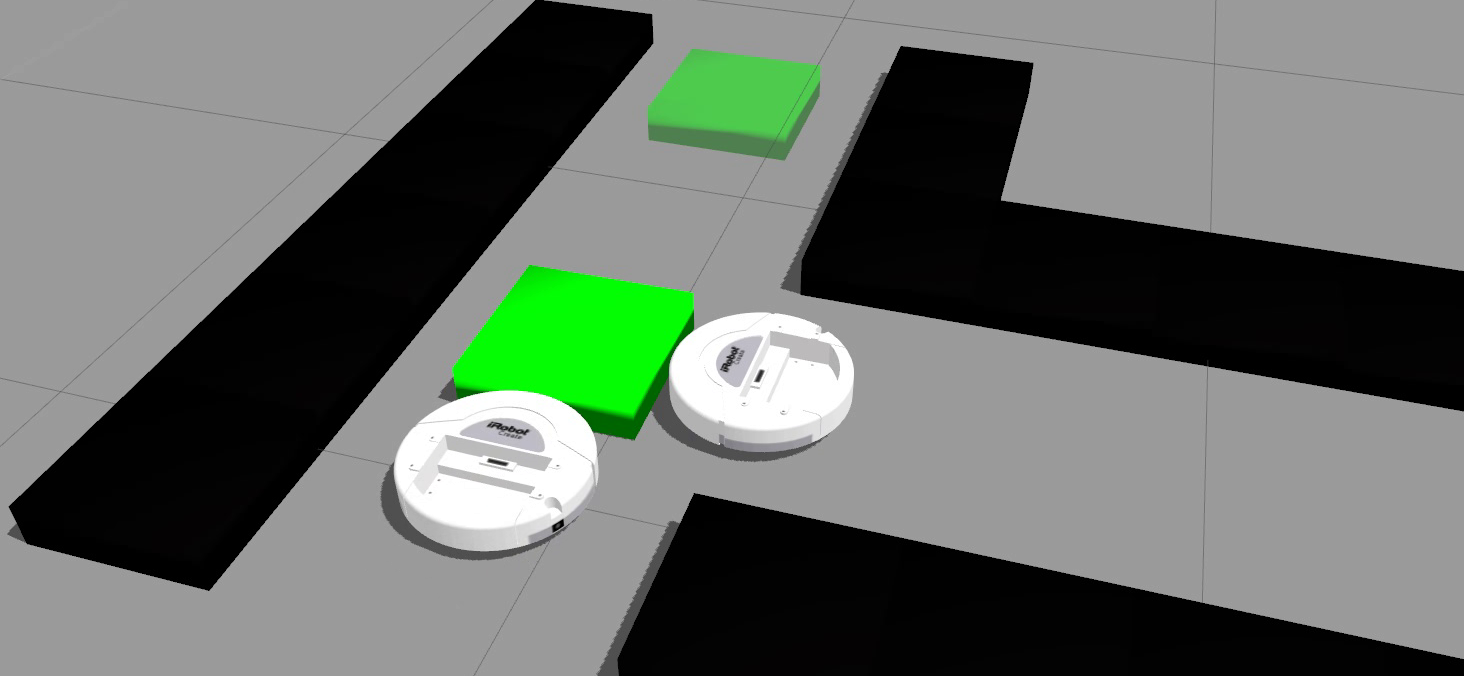
\includegraphics[width=\textwidth]{img/experimentos/sim_200.png}}
    \caption{t=200s}
    \label{fig:sim_200}
  \end{subfigure}

  \begin{subfigure}[t]{0.45\textwidth}
    \centering
    \fbox{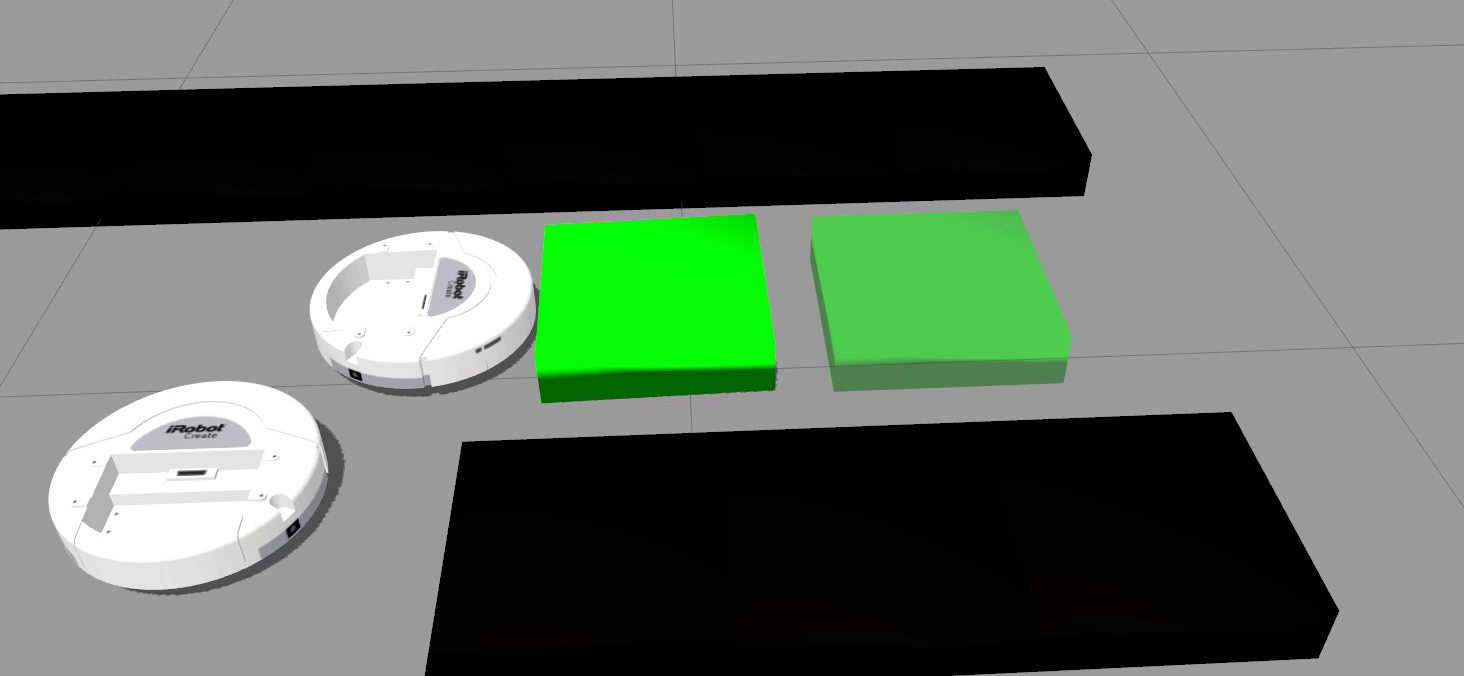
\includegraphics[width=\textwidth]{img/experimentos/sim_230.png}}
    \caption{t=230s}
    \label{fig:sim_230}
  \end{subfigure}
  \hspace{0.2cm}
  \begin{subfigure}[t]{0.45\textwidth}
    \centering
    \fbox{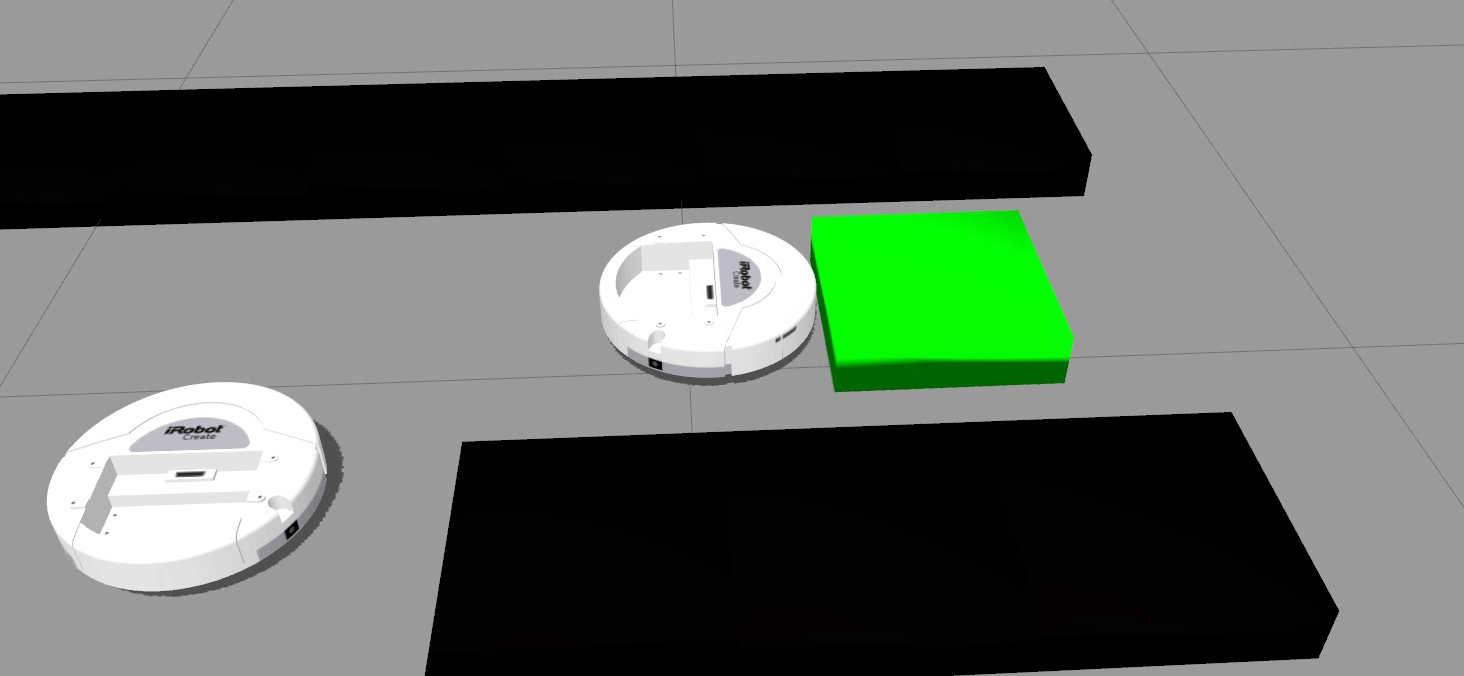
\includegraphics[width=\textwidth]{img/experimentos/sim_250.png}}
    \caption{t=250s}
    \label{fig:sim_250}
  \end{subfigure}

  \caption{Exemplo de transporte por dois agentes em um ambiente simulado.}
  \label{fig:sim_ground}

\end{figure}

Neste exemplo de execução, o agente mais próximo do objeto será alocado para realizar o primeiro segmento do transporte do objeto através do corredor formado pelos obstáculos (figuras \ref{fig:sim_1} a \ref{fig:sim_139}).
Considerando que para continuar a execução do transporte, o primeiro agente deve andar uma grande distância, o segundo agente assume o objeto para realização do segundo segmento, levando-o até a posição final, demarcada por uma caixa verde semitransparente (figuras \ref{fig:sim_180} a \ref{fig:sim_250}).

No outro ambiente simulado apresentado na Figura \ref{fig:sim_aerial}, é demonstrado o transporte do objeto em questão utilizando agentes de tipos diferentes, um terrestre, da mesma plataforma utilizada anteriormente (\emph{iRobot Create}), e um aéreo, que é representado por um robô genérico no modelo \emph{quadrotor}, este tipo de agente foi escolhido por sua capacidade de pairar, sendo capaz de pegar o objeto ainda no ar utilizando a ação de \emph{GRASP}.

Diferente do ambiente anterior, neste novo cenário o objeto não tem acesso direto ao seu destino por vías terrestres, sendo necessário o uso do agente aéreo.
Em um primeiro momento, visto nas figuras \ref{fig:sim_aerial_1} até \ref{fig:sim_aerial_668}, o agente terrestre transporta o objeto até o local mais próximo possível de sua posição final evitando o objeto colida com os obstáculos, em seguida (figuras \ref{fig:sim_aerial_687} a \ref{fig:sim_aerial_742}) o agente aéreo é acionado, indo até a posição atual do objeto, realiza a ação de \emph{GRASP} e o leva até a pose final designada.

\begin{figure}[ht!]
  \centering
  \setlength{\fboxsep}{0pt}

  \begin{subfigure}[t]{0.45\textwidth}
    \centering
    \fbox{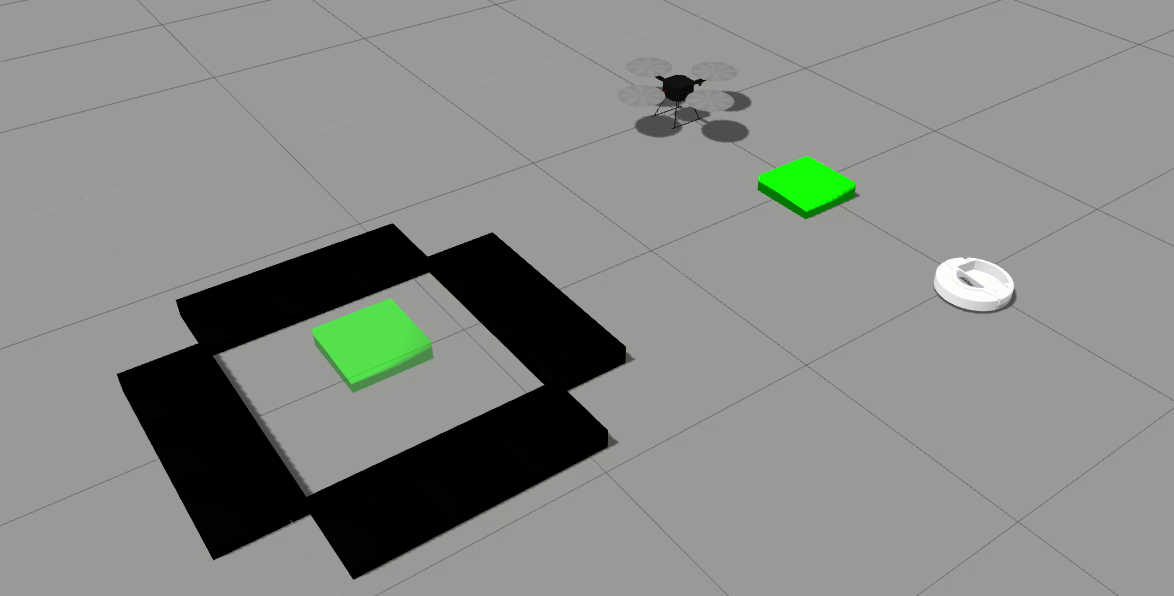
\includegraphics[width=\textwidth]{img/experimentos/sim_aerial/sim_001.png}}
    \caption{t=1s}
    \label{fig:sim_aerial_1}
  \end{subfigure}
  \hspace{0.2cm}
  \begin{subfigure}[t]{0.45\textwidth}
    \centering
    \fbox{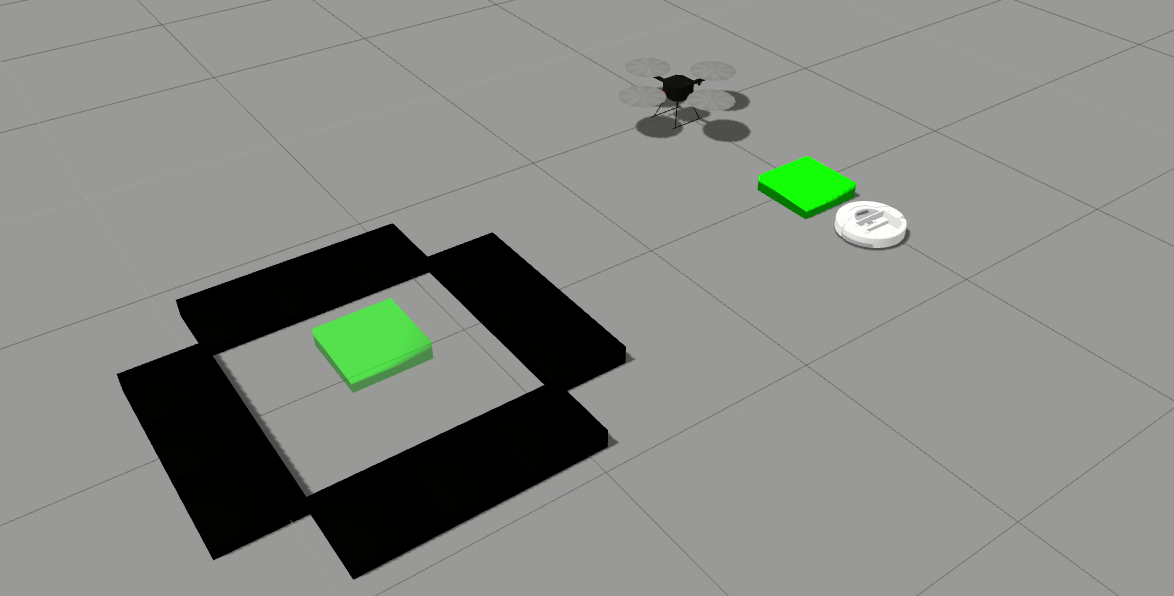
\includegraphics[width=\textwidth]{img/experimentos/sim_aerial/sim_139.png}}
    \caption{t=139s}
    \label{fig:sim_aerial_139}
  \end{subfigure}

  \begin{subfigure}[t]{0.45\textwidth}
    \centering
    \fbox{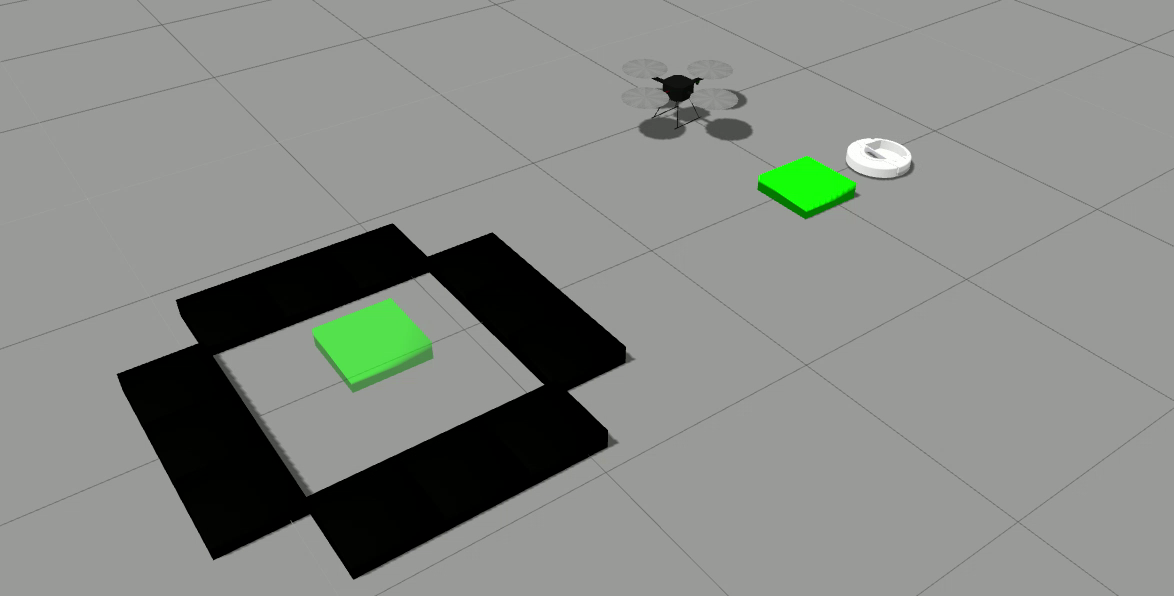
\includegraphics[width=\textwidth]{img/experimentos/sim_aerial/sim_459.png}}
    \caption{t=459s}
    \label{fig:sim_aerial_459}
  \end{subfigure}
  \hspace{0.2cm}
  \begin{subfigure}[t]{0.45\textwidth}
    \centering
    \fbox{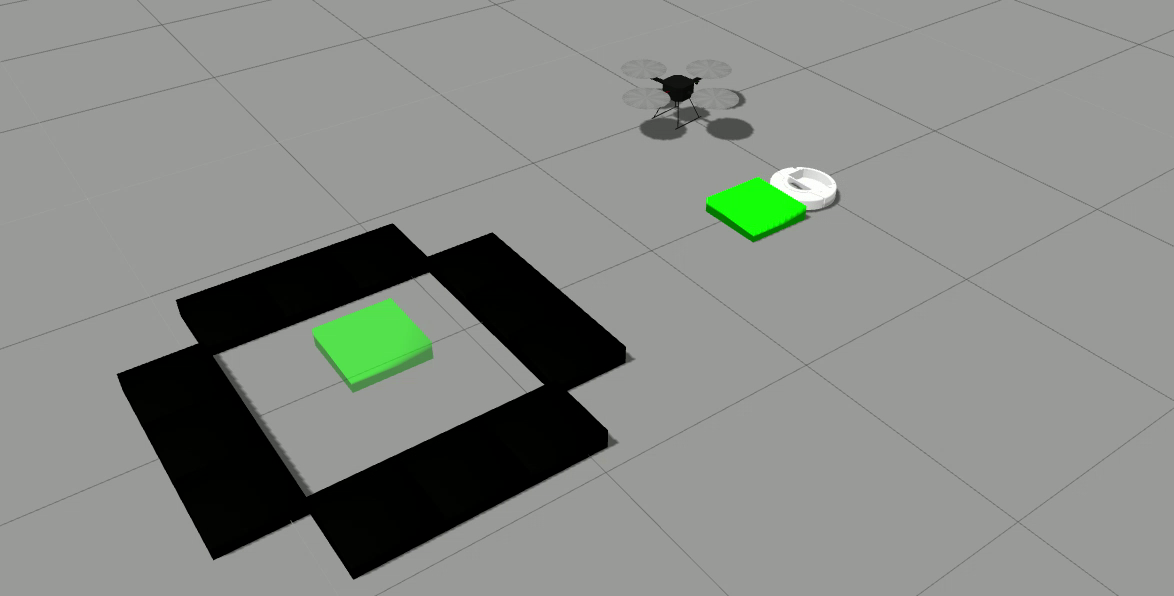
\includegraphics[width=\textwidth]{img/experimentos/sim_aerial/sim_566.png}}
    \caption{t=566s}
    \label{fig:sim_aerial_566}
  \end{subfigure}

  \begin{subfigure}[t]{0.45\textwidth}
    \centering
    \fbox{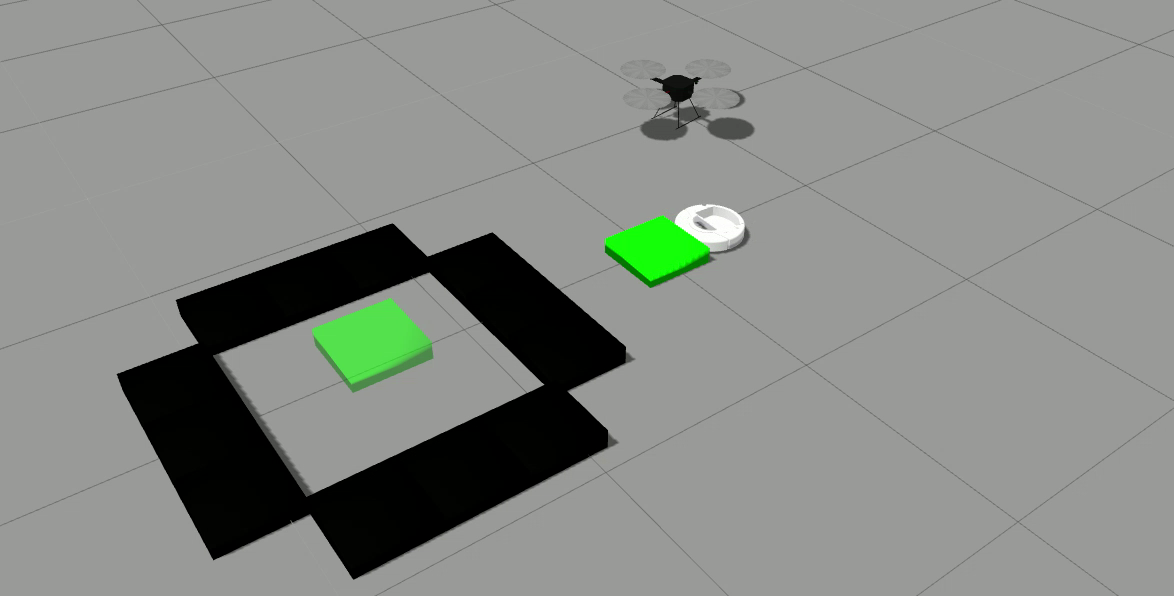
\includegraphics[width=\textwidth]{img/experimentos/sim_aerial/sim_668.png}}
    \caption{t=668s}
    \label{fig:sim_aerial_668}
  \end{subfigure}
  \hspace{0.2cm}
  \begin{subfigure}[t]{0.45\textwidth}
    \centering
    \fbox{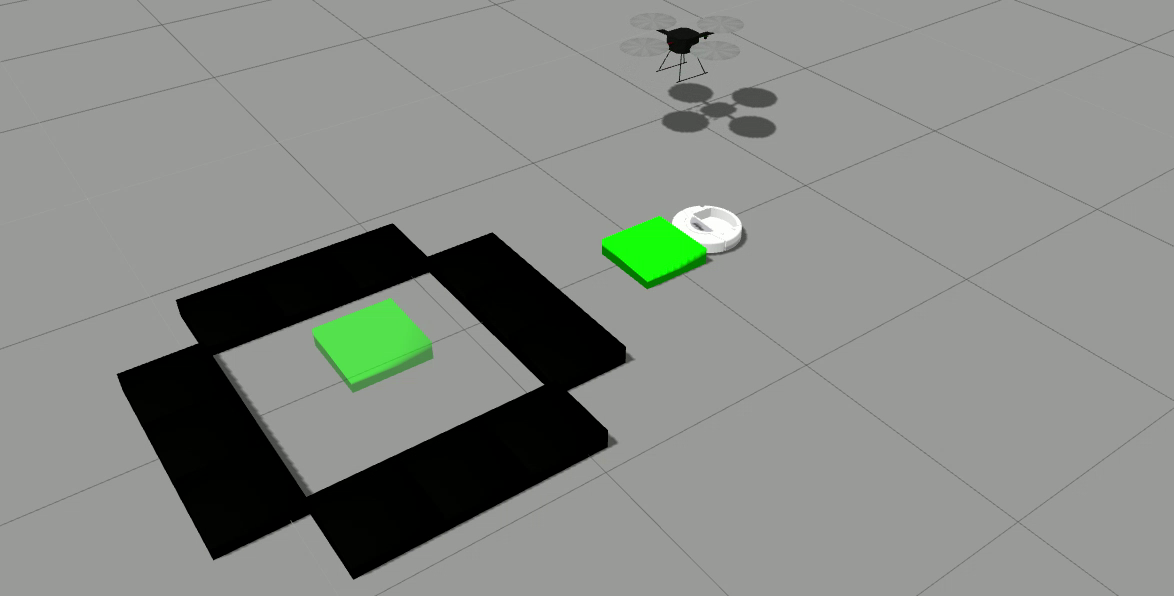
\includegraphics[width=\textwidth]{img/experimentos/sim_aerial/sim_687.png}}
    \caption{t=687s}
    \label{fig:sim_aerial_687}
  \end{subfigure}

  \begin{subfigure}[t]{0.45\textwidth}
    \centering
    \fbox{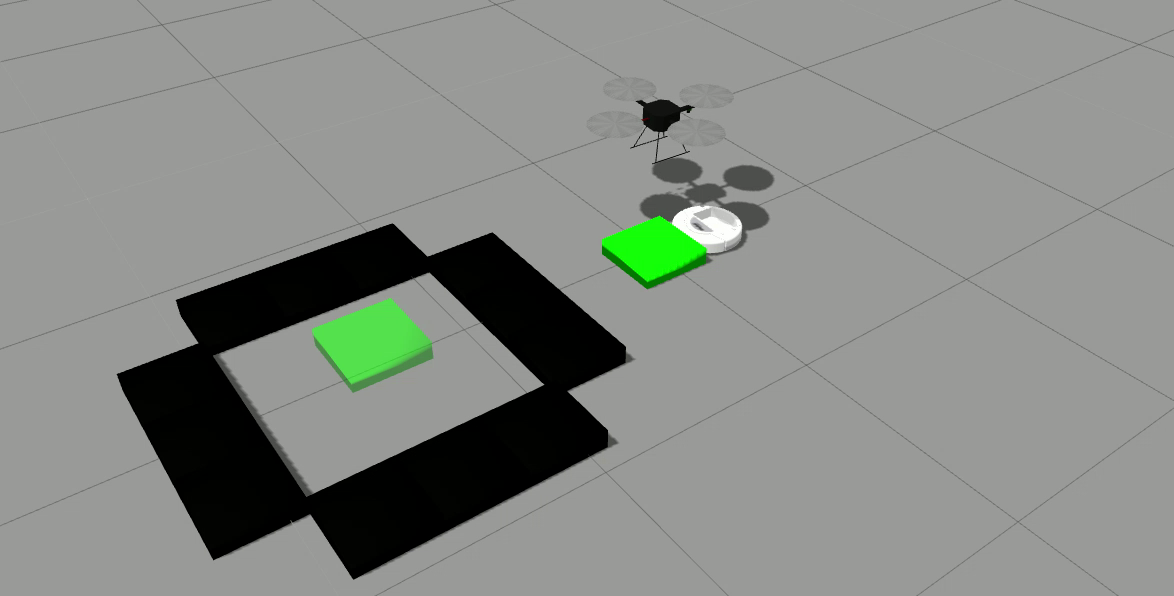
\includegraphics[width=\textwidth]{img/experimentos/sim_aerial/sim_700.png}}
    \caption{t=700s}
    \label{fig:sim_aerial_700}
  \end{subfigure}
  \hspace{0.2cm}
  \begin{subfigure}[t]{0.45\textwidth}
    \centering
    \fbox{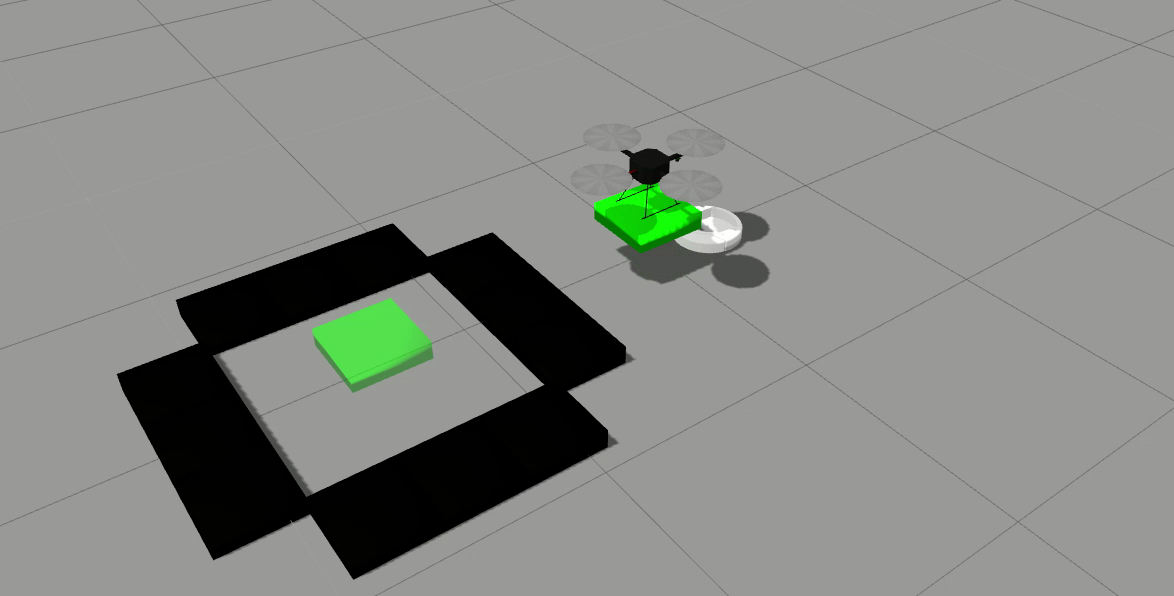
\includegraphics[width=\textwidth]{img/experimentos/sim_aerial/sim_713.png}}
    \caption{t=713s}
    \label{fig:sim_aerial_713}
  \end{subfigure}

  \begin{subfigure}[t]{0.45\textwidth}
    \centering
    \fbox{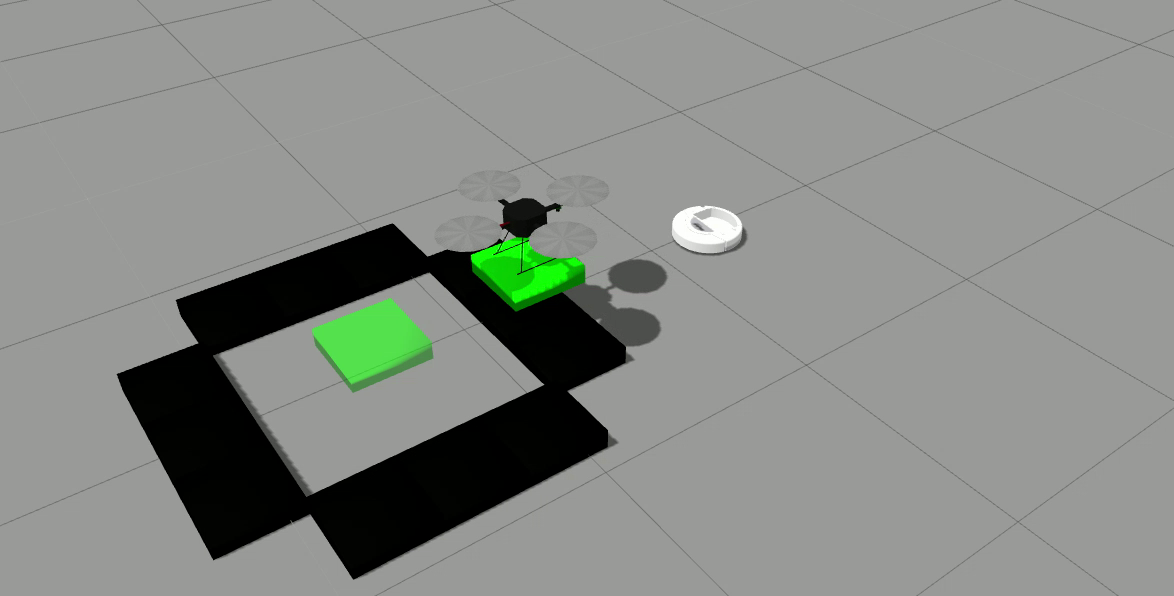
\includegraphics[width=\textwidth]{img/experimentos/sim_aerial/sim_720.png}}
    \caption{t=720s}
    \label{fig:sim_aerial_720}
  \end{subfigure}
  \hspace{0.2cm}
  \begin{subfigure}[t]{0.45\textwidth}
    \centering
    \fbox{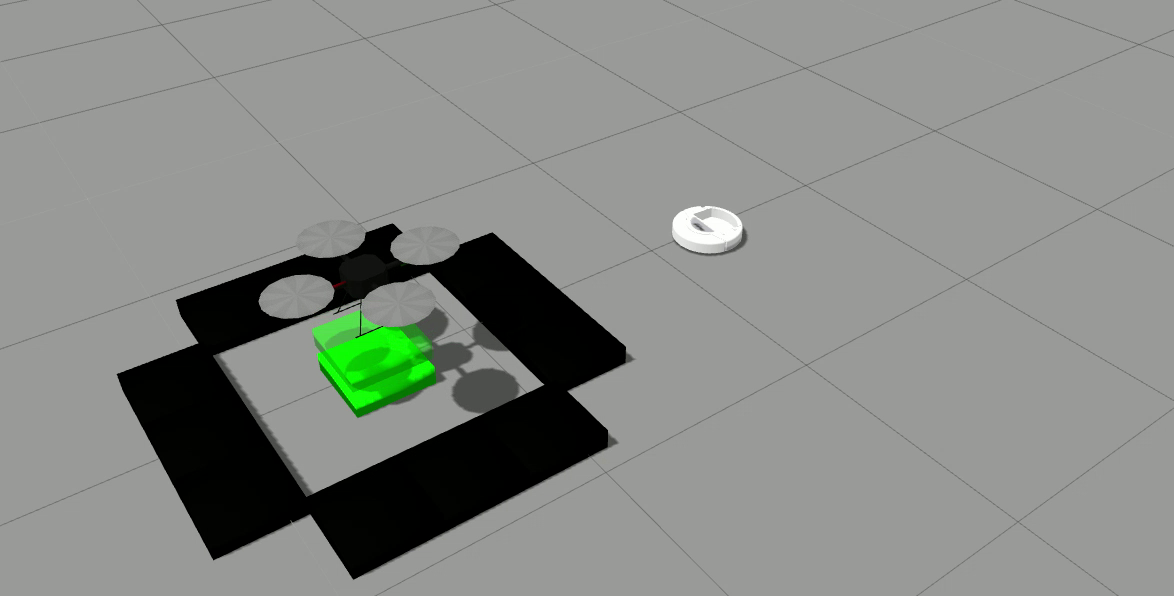
\includegraphics[width=\textwidth]{img/experimentos/sim_aerial/sim_742.png}}
    \caption{t=742s}
    \label{fig:sim_aerial_742}
  \end{subfigure}

  \caption{Exemplo de transporte utilizando um agente terrestre e um aéreo.}
  \label{fig:sim_aerial}

\end{figure}

Mediante estes exemplos, é possível ver todas as etapas anteriormente discutidas, havendo o planejamento para o objeto, os agentes realizam seus próprios planejamento e se coordenam de modo a transportar o objeto da melhor maneira possível, respeitando as restrições impostas pelo ambiente.

% Algoritmo de Controle

O controle dos agentes durante a movimentação no ambiente de trabalho foi realizado utilizando um conjunto de algoritmos separados em dois níveis: (i) controlador de navegação, que mantém um registro de todas as posições no ambiente de trabalho que o agente deve percorrer para completar o plano previamente criado, além de gerenciar o envio de novos pontos de destino sempre que detectar a chegada do agente a uma posição previamente enviada; (ii) controlador de velocidades, este recebe um ponto de destino do controlador de navegação, e baseado na posição atual do agente, aplica um controlador PI (proporcional-integrativo) para realizar a movimentação do agente para a posição requerida.

Para ambos os agentes, o algoritmo do controlador de navegação utilizado é o mesmo, pois é necessário somente o repasse dos pontos de destino, porém o controlador de baixo nível (velocidades) é diferenciado, considerando que os agentes possuem maneiras de movimentação distintas.
Os Algoritmos \ref{alg:aerial_vel} e \ref{alg:land_vel} demonstram sucintamente estes controladores, respectivamente do agente aéreo e terrestre.

\begin{algorithm}[h]
  \caption{AerialVelocityController(goal\_pose, last\_cmd, vertical\_lim, P, I)}
  \label{alg:aerial_vel}
  \begin{algorithmic}[1]
    \STATE{current\_pose $\leftarrow$ get\_current\_pose()}
    \STATE{current\_orientation $\leftarrow$ get\_orientation(current\_pose)}
    \STATE{}
    \STATE{diff\_x $\leftarrow$ goal\_pose[x] - current\_pose[x]}
    \STATE{diff\_y $\leftarrow$ goal\_pose[y] - current\_pose[y]}
    \STATE{diff\_z $\leftarrow$ goal\_pose[z] - current\_pose[z]}
    \STATE{}
    \STATE{angular\_vel $\leftarrow$ P * current\_orientation + I * last\_cmd[angle]}
    \STATE{}
    \IF{abs(diff\_z) $>$ vertical\_lim}
      \STATE{linear\_vel\_x $\leftarrow 0$}
      \STATE{linear\_vel\_y $\leftarrow 0$}
    \ELSE
      \STATE{linear\_vel\_x $\leftarrow$ P * diff\_x + I * last\_cmd[x]}
      \STATE{linear\_vel\_y $\leftarrow$ P * diff\_y + I * last\_cmd[y]}
    \ENDIF
    \STATE{linear\_vel\_z $\leftarrow$ P * diff\_z + I * last\_output[z]}
    \RETURN{[linear\_vel\_x, linear\_vel\_y, linear\_vel\_z, angular\_vel]}
  \end{algorithmic}
\end{algorithm}

\begin{algorithm}[h]
  \caption{AerialVelocityController(goal\_pose, last\_cmd, angular\_lim, P, I)}
  \label{alg:land_vel}
  \begin{algorithmic}[1]
    \STATE{current\_pose $\leftarrow$ get\_current\_pose()}
    \STATE{current\_orientation $\leftarrow$ get\_orientation(current\_pose)}
    \STATE{}
    \STATE{diff\_orientation $\leftarrow$ angle\_between\_poses(current\_pose, goal\_pose)}
    \STATE{diff\_distance $\leftarrow$ distance\_between\_poses(current\_pose, goal\_pose)}
    \STATE{}
    \IF{abs(diff\_orientation) $>=$ angular\_lim}
      \STATE{linear\_vel $\leftarrow 0$}
    \ELSE
      \STATE{linear\_vel $\leftarrow$ P * diff\_distance + I * last\_cmd[linear]}
    \ENDIF
    \STATE{angular\_vel $\leftarrow$ P * diff\_orientation + I * last\_cmd[angular]}
    \RETURN{[linear\_vel, angular\_vel]}
  \end{algorithmic}
\end{algorithm}

O Algoritmo \ref{alg:aerial_vel}, demonstra o controle para o agente aéreo.
Em um primeiro momento, o mesmo guarda referências para sua posição e orientação atual (referente ao sistema de coordenada do mundo), e calcula a diferença entre sua atual localidade até o ponto de destino.
Considerando que não há necessidade de rotação do agente, o mesmo deve manter uma orientação fixa próximo ao valor $0$, assim é calculada a velocidade angular necessária para correção de possíveis variações (linha $8$).
Nas demais linhas, são calculas as velocidades lineares de movimentação em três dimensões (x, y, z), observando para um detalhe na linha 10, que faz uso da constante $vertical\_lim$ para delimitar uma distância mínima entre a altitude do agente e a altitude de destino, fazendo com o mesmo se movimente no plano (x, y) somente quando este limiar for atingido.
Sem este detalhe de implementação, o agente movimentáva-se nos três eixos simultaneamente, ocasionando em colisões descenessárias com o ambiente.

Para o agente terrestre, foi utilizado o Algoritmo \ref{alg:land_vel}, que funciona de forma similar ao demonstrado anteriormente, porém de forma mais simples. Baseado na posição e orientação atual, o agente calcula a diferença de ângulo até o ponto de destino, aplicando a função $\arctan$, além da distância entre os mesmos.
Análogo ao limiar de altitude, o agente terrestre utiliza a constante $angular\_lim$ para delimitar uma diferença de angulo mínimo para que o robô possa se mover. Durante os testes, fora utilizado um valor reduzido para tal constante, ocasionando em uma ausência de curvas por parte do agente, de modo que o mesmo primeiramente realiza um alinhamento em direção à posição de destino e só então realiza a movimentação.

Em ambos os algoritmos, os valores passados através variável $last\_cmd$, são todos aqueles calculados durante a ultima iteração do mesmo, controlado externamento pelo algoritmo de navegação.

\subsection{Ambiente Real} % (fold)
\label{sub:ambiente_real}

Os experimentos reais foram realizados utilizando somente agentes terrestres, em um espaço de área aproximada de 2m x 2m situado no laboratório de Visão Computacional e Robótica (VeRLab)\footnote{\url{http://www.verlab.dcc.ufmg.br/}}.
O mesmo controlador anteriormente descrito foi utilizado, com pequenos ajustes nos valores das constantes para atender às variações do ambiente real.

A metodologia apresentada considera que a localização de todos os agentes, objetos e obstáculos no ambiente é conhecida durante a missão de transporte, para tanto, a localização de tais itens foi realizada utilizando marcadores fiduciais que identificam unicamente cada um e são reconhecidos por uma câmera posicionada acima da área de trabalho, sendo capaz de detectar a posição de cada marcador e informar ao sistema estas informações em tempo real.

A plataforma robótica utilizada nos experimentos é do modelo \emph{ePuck}\footnote{\url{http://www.e-puck.org/}}, robô diferencial, com 70mm de diâmetro e 150g, controlado através de comunicação \emph{bluetooth}.
Esta robô é capaz de se movimentar, além de possuir alguns sensores, como uma câmera, um conjunto de infra-vermelhos para detecção de obstáculos, além de \emph{encoders} para as rodas.
A Figura \ref{fig:epucks} exemplifica o agente utilizado durante o experimentos.

O ambiente de trabalho montado para realização deste experimento consistia na utilização de três robôs \emph{ePuck}s, um objeto a ser transportado, e um conjunto arbitrário de obstáculos dispostos no ambiente, como é demonstrado na Figura \ref{fig:real_workspace}.
Como apresentado na figura, os agentes foram colocados em uma região à parte do ambiente, passíveis de serem utilizados durante o transporte.
O objeto a ser transportado é considerado possuindo peso e resistência desprezíveis, por ser constituído de uma espuma de baixa densidade e apresentar baixa taxa atrito com a superfície na qual o teste está sendo realizado, além de possuir a mesma dimensão (largura e comprimento) que os agentes.
Os agentes tem por objetivo levar o objeto de sua posição inicial, assinala em verde, para a posição final, destacada em vermelho.

A Figura \ref{fig:real} demonstra a execução da missão de transporte pelos três agentes, considerando que as etapas de planejamento de caminhos do objetos (destacada pelo caminho na cor branca na Figura \ref{fig:real_workspace}, possuindo 3 segmentos) e dos agentes, além da alocação de tarefas já foram realizadas enquanto os agentes permaneciam em suas respectivas posições iniciais.
Como pode ser observado, o agente 1 é selecionado para iniciar o transporte, enquanto os demais agentes se movimentam para esperar sua vez.
Assim que o agente transporta objeto através do primeiro segmento (S1) na Figura \ref{fig:real_5} o agente 2 torna-se o responsável pelo transporte através do segmento S2, até que a missão é repassada para o agente 3 como demonstrado na Figura \ref{fig:real_7}, que termina a movimentação do objeto até a posição final passando pelo segmento S3.

\begin{figure}[h]
  \centering
  \setlength{\fboxsep}{0pt}
  \fbox{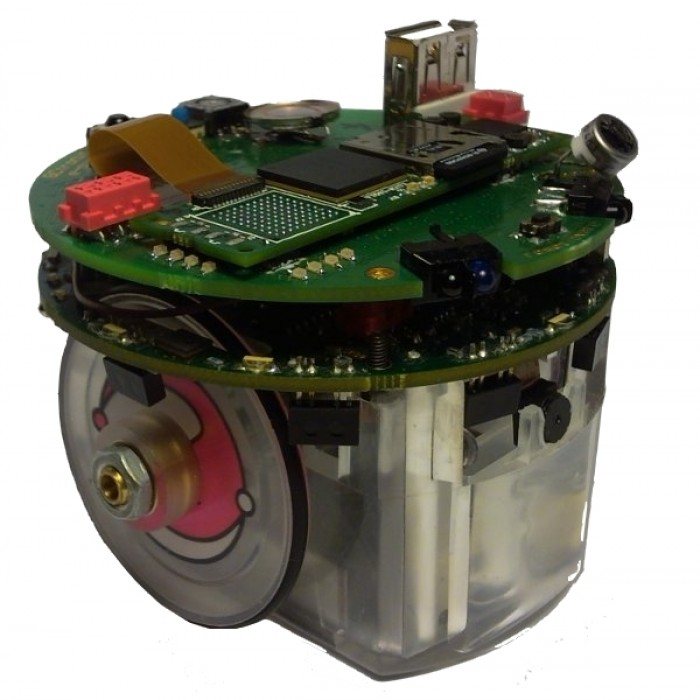
\includegraphics[width=0.44\textwidth]{img/experimentos/epuck.jpg}}
  \caption{Plataforma robótica ePuck utilizada durante os experimentos reais.}
  \label{fig:epucks}
\end{figure}

\begin{figure}[h]
  \centering
  \setlength{\fboxsep}{0pt}
  \fbox{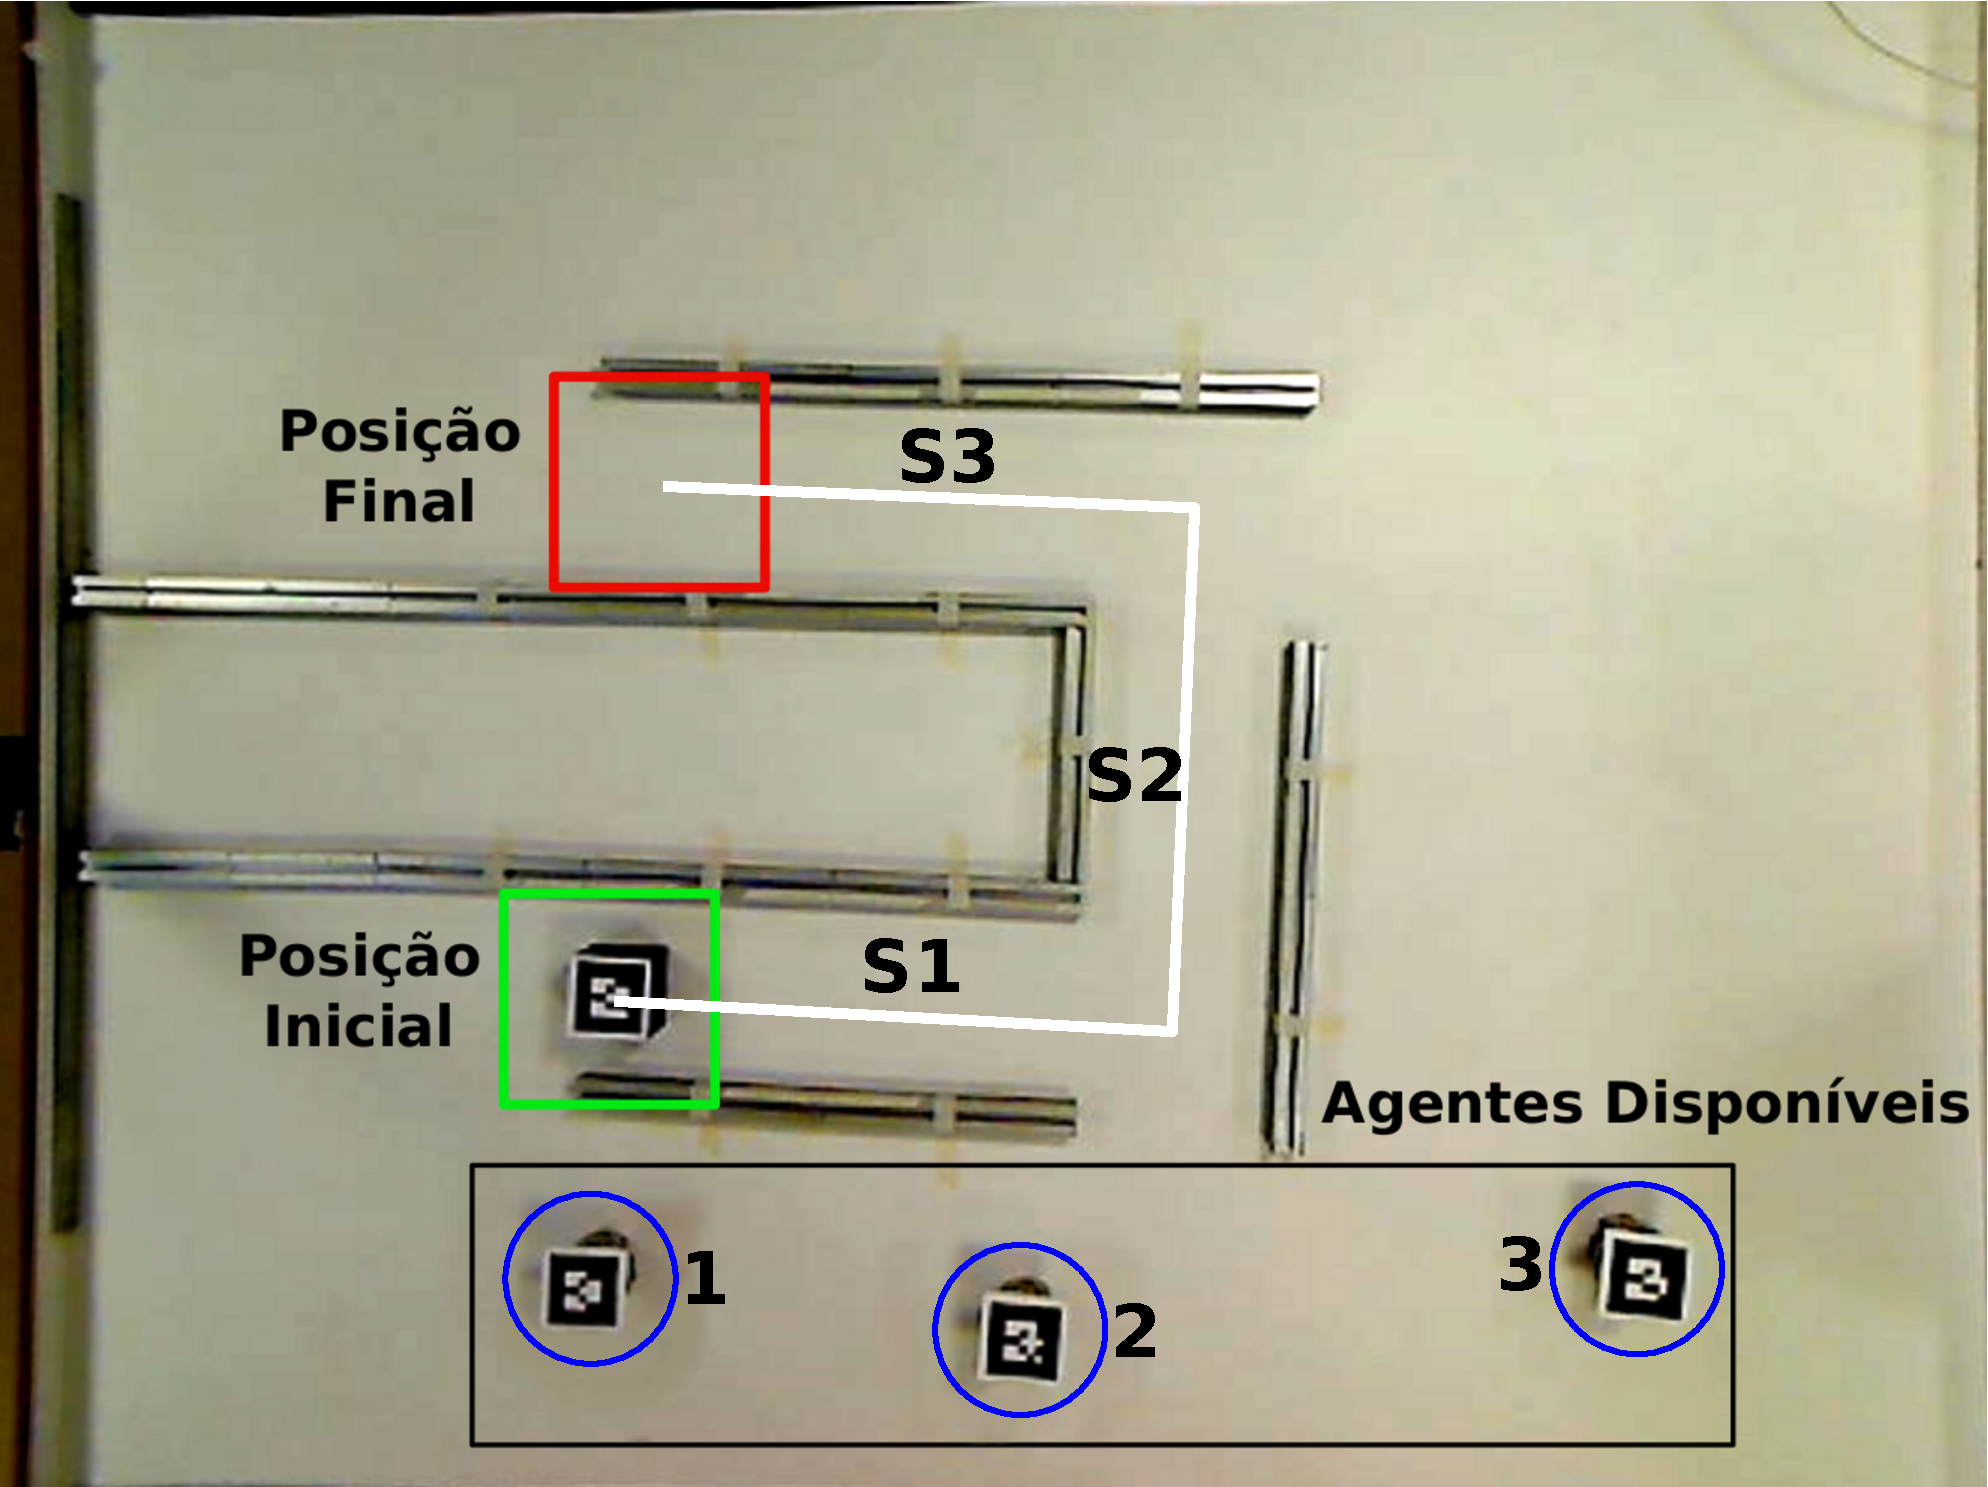
\includegraphics[width=0.85\textwidth]{img/experimentos/experiment_real.pdf}}
  \caption{Configuração do ambiente de trabalho no experimento real.}
  \label{fig:real_workspace}
\end{figure}

\begin{figure}[htpb]
  \centering
  \setlength{\fboxsep}{0pt}

  \begin{subfigure}[t]{0.45\textwidth}
    \centering
    \fbox{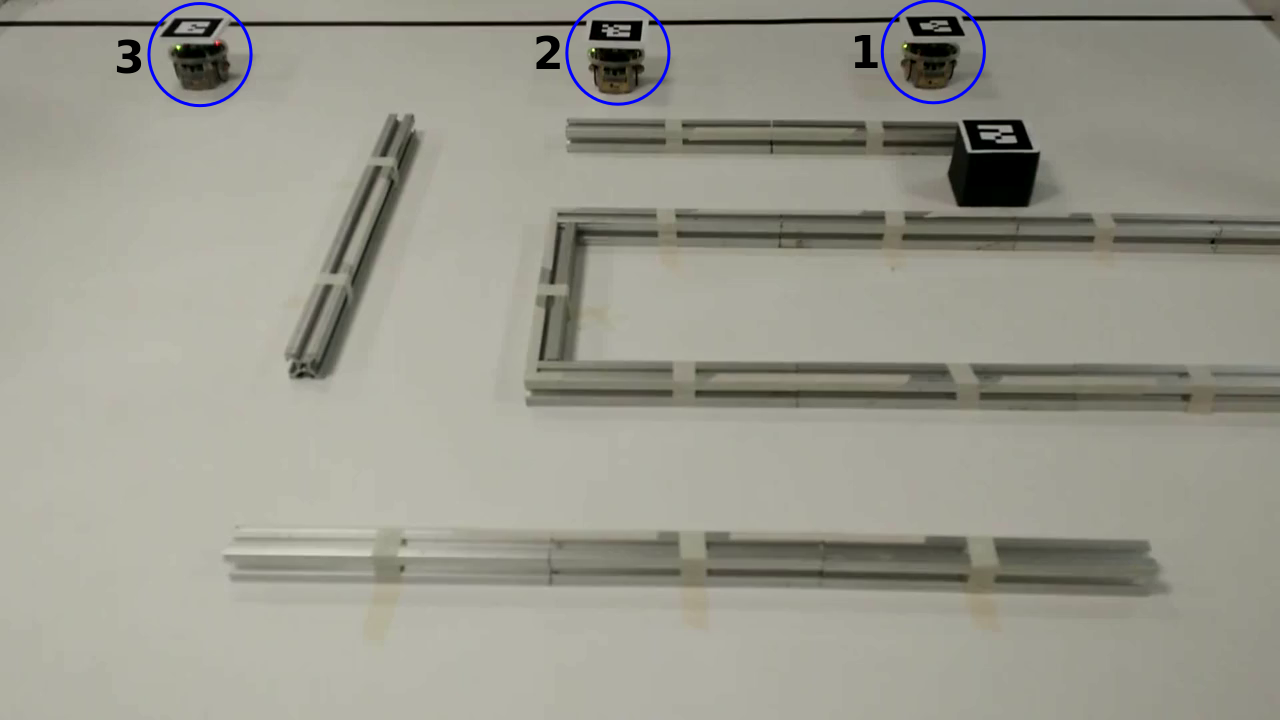
\includegraphics[width=\textwidth]{img/experimentos/real1_1.png}}
    \caption{t=1s}
    \label{fig:real_1}
  \end{subfigure}
  \hspace{0.2cm}
  \begin{subfigure}[t]{0.45\textwidth}
    \centering
    \fbox{\includegraphics[width=\textwidth]{img/experimentos/real2.png}}
    \caption{t=24s}
    \label{fig:real_2}
  \end{subfigure}

  \begin{subfigure}[t]{0.45\textwidth}
    \centering
    \fbox{\includegraphics[width=\textwidth]{img/experimentos/real3.png}}
    \caption{t=72s}
    \label{fig:real_3}
  \end{subfigure}
  \hspace{0.2cm}
  \begin{subfigure}[t]{0.45\textwidth}
    \centering
    \fbox{\includegraphics[width=\textwidth]{img/experimentos/real4.png}}
    \caption{t=102s}
    \label{fig:real_4}
  \end{subfigure}

  \begin{subfigure}[t]{0.45\textwidth}
    \centering
    \fbox{\includegraphics[width=\textwidth]{img/experimentos/real5.png}}
    \caption{t=150s}
    \label{fig:real_5}
  \end{subfigure}
  \hspace{0.2cm}
  \begin{subfigure}[t]{0.45\textwidth}
    \centering
    \fbox{\includegraphics[width=\textwidth]{img/experimentos/real6.png}}
    \caption{t=180s}
    \label{fig:real_6}
  \end{subfigure}

  \begin{subfigure}[t]{0.45\textwidth}
    \centering
    \fbox{\includegraphics[width=\textwidth]{img/experimentos/real7.png}}
    \caption{t=216s}
    \label{fig:real_7}
  \end{subfigure}
  \hspace{0.2cm}
  \begin{subfigure}[t]{0.45\textwidth}
    \centering
    \fbox{\includegraphics[width=\textwidth]{img/experimentos/real8.png}}
    \caption{t=258s}
    \label{fig:real_8}
  \end{subfigure}

  \begin{subfigure}[t]{0.45\textwidth}
    \centering
    \fbox{\includegraphics[width=\textwidth]{img/experimentos/real9.png}}
    \caption{t=282s}
    \label{fig:real_9}
  \end{subfigure}
  \hspace{0.2cm}
  \begin{subfigure}[t]{0.45\textwidth}
    \centering
    \fbox{\includegraphics[width=\textwidth]{img/experimentos/real10.png}}
    \caption{t=306s}
    \label{fig:real_10}
  \end{subfigure}

  \caption{Exemplo de transporte de um objeto utilizando três agentes reais.}
  \label{fig:real}

\end{figure}

% subsection ambiente_real (end)

% chapter experimentos (end)
